
\usepackage{graphicx} % Required for inserting images

\documentclass[11pt]{article}
\usepackage[hmargin=1in,vmargin=1in]{geometry}
\usepackage{xcolor}
\usepackage{amsmath,amssymb,amsfonts,url,sectsty,framed,tcolorbox,framed}
\usepackage{nicematrix}
\usepackage{algorithm2e}
\setcounter{MaxMatrixCols}{16}
\usepackage{tikz}
\usepackage{hyperref}
\usetikzlibrary{decorations.pathreplacing}
\newcommand{\pf}{{\bf Proof: }}
\newtheorem{theorem}{Theorem}
\newtheorem{lemma}{Lemma}
\newtheorem{proposition}{Proposition}
\newtheorem{definition}{Definition}
\newtheorem{remark}{Remark}
\newcommand{\qed}{\hfill \rule{2mm}{2mm}}
\usepackage{titlesec}

\setcounter{secnumdepth}{4}
\titleclass{\subsubsubsection}{straight}[\subsection]
\newcounter{subsubsubsection}[subsubsection]
\renewcommand{\thesubsubsubsection}{\thesubsubsection.\arabic{subsubsubsection}}
\titleformat{\subsubsubsection}{\normalfont\normalsize\bfseries}{\thesubsubsubsection}{1em}{}
\titlespacing*{\subsubsubsection}{0pt}{3.25ex plus 1ex minus .2ex}{1.5ex plus .2ex}

\setcounter{tocdepth}{4}

\begin{document}



%%%%%%%%%%%%%%%%%%%%%%%%%%%%%%%%%%%%%%%%%%%%%%%%%%%%%%%%%%%%%%%%%%%%%
\noindent
\rule{\textwidth}{1pt}
\begin{center}
{\bf [CS304] Introduction to Cryptography and Network Security}
\end{center}
Course Instructor: Dr. Dibyendu Roy \hfill Winter 2022-2023\\
Scribed by: Chitranshi Srivastava (202051055) \hfill Lecture 15, 16, 17 and 18(Week 8 and 9)
\\
\rule{\textwidth}{1pt}
%%%%%%%%%%%%%%%%%%%%%%%%%%%%%%%%%%%%%%%%%%%%%%%%%%%%%%%%%%%
%write here

\section{One Time Padding}
As we have discussed earlier, so we know encryption and decryption in OTP are given as:\\
    \textbf{Encryption:} $C = M \oplus K$\\
    \textbf{Decryption:} $M = C \oplus K$\\ 
We have already discussed that OTP provides perfect secrecy under the following conditions:
\begin{enumerate}
    \item The secret key K cannot be used to encrypt two messages, that is, the key can not be reused.
    \item The length of key must be greater than or equal to the length of message.
    \item Key K is uniformly selected from the key space.
\end{enumerate}

However, OTP is not practical because if we have a method to share the secret key (length equal to the message), then we can share the message using that mechanism. Here, we want to design an algorithm as efficient as OTP but which can be used for practical purposes. Also, it may not provide perfect secrecy, but it is not possible to prove or disprove that it provides perfect secrecy.\\
\vspace{3mm}
Let us a define a function F as:
\begin{center}
    $F(K, IV) = Z_i$ where $Z_i \in \{0, 1\}$
\end{center}
K is secret key, IV is initialization vector (a public parameter). Function F produces n bits $Z_0, Z_1,....., Z_{n-1}$. The function F is efficiently computable.\\
    \textbf{Plaintext:} $m_0, m_1,....., m_{n-1}$\\
    \textbf{Z:} $Z_0, Z_1,....., Z_{n-1}$\\
    \textbf{Encryption:} $C_0 = m_0 \oplus Z_0, C_1 = m_1 \oplus Z_1,....., C_{n-1} = m_{n-1} \oplus Z_{n-1}$\\

The function F, known as Pseudo Random Bit Generation Function has certain properties. These properties are listed below:
\begin{enumerate}
    \item The output i.e. $Z_0, Z_1,....., Z_{n-1}$ is a random looking string. Let us try to understand the meaning of random looking string. Consider an unbiased coin, toss it for n times, output 0 if head comes, and 1 if tails comes up. Let's say the string generated by coin tossing is $x_0, x_1,....., x_{n-1}$. Now if you are given the string $Z_0, Z_1,....., Z_{n-1}$, you cannot distinguish, whether the string is obtained from a coin tossing experiment or by a pseudo random bit generator with key and IV as input. However, the string $Z_0, Z_1,....., Z_{n-1}$ can be reproduced by passing the same inputs to the function F. This means a string that seems to be random but can be reproduced again by passing same inputs to F is known as random looking string.
    \item If we give same input (K, IV) to F in different time, it will generate same $Z_i$.

    \begin{center}
        \tikzset{every picture/.style={line width=0.75pt}} 
        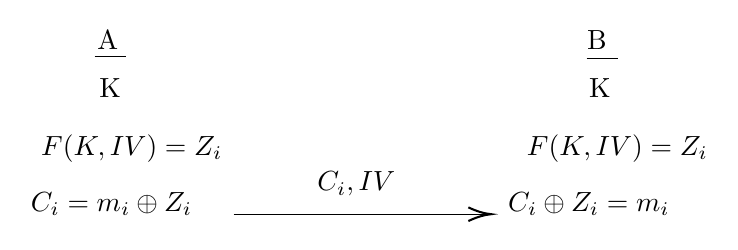
\begin{tikzpicture}[x=0.75pt,y=0.75pt,yscale=-1,xscale=1]
            \draw    (139,71.6) -- (154,71.6) ;
            \draw    (376,72.6) -- (391,72.6) ; 
            \draw    (206,147.6) -- (328,147.6) ;
            \draw [shift={(330,147.6)}, rotate = 180] [color={rgb, 255:red, 0; green, 0; blue, 0 }  ][line width=0.75]    (10.93,-3.29) .. controls (6.95,-1.4) and (3.31,-0.3) .. (0,0) .. controls (3.31,0.3) and (6.95,1.4) .. (10.93,3.29)   ;
            
            \draw (139,58) node [anchor=north west][inner sep=0.75pt]   [align=left] {A};
            \draw (375,58) node [anchor=north west][inner sep=0.75pt]   [align=left] {B};
            \draw (140,81) node [anchor=north west][inner sep=0.75pt]   [align=left] {K};
            \draw (376,81) node [anchor=north west][inner sep=0.75pt]   [align=left] {K};
            \draw (112,108) node [anchor=north west][inner sep=0.75pt]   [align=left] {$F(K,IV) = Z_i$};
            \draw (346,108) node [anchor=north west][inner sep=0.75pt]   [align=left] {$F(K,IV) = Z_i$};
            \draw (107,136) node [anchor=north west][inner sep=0.75pt]   [align=left] {$C_i = m_i \oplus Z_i$};
            \draw (337,136) node [anchor=north west][inner sep=0.75pt]   [align=left] {$C_i \oplus Z_i = m_i$};
            \draw (245,126) node [anchor=north west][inner sep=0.75pt]   [align=left] {$C_i, IV$};
        \end{tikzpicture}
    \end{center}    

    \item If key K is selected randomly and is kept secret, then the outputs $Z_0, Z_1,....., Z_{n-1}$ will be indistinguishable from bit string generated by using a random bit generator (coin tossing).
    \begin{center}
        $F(K, IV) \rightarrow Z_0, Z_1,....., Z_{n-1}$ and Coin Tossing $\rightarrow x_0, x_1,....., x_{n-1}$ are indistinguishable.
    \end{center}

    \item The length of the output bits $Z_0, Z_1,....., Z_{n-1}$, that is, $n$ is very much larger than the length of K. There are efficient functions that can produce $2^{80} - 1$ length output for a key of length 80 bits. Using this property, a small key can encrypt very large messages. However, if there is repetition in the output bits, then difference can be calculated between corresponding message bits just as in OTP. Block ciphers like AES and DES will take a very long time to encrypt a message of $2^{80} - 1$ bits. DES will perform around $2^{64}$ encryption to encrypt the whole message. Hence, this technique is much more efficient.

    \item If we modify at least one bit of K or of IV, then there will be unpredictable change in output of $Z_i$. 
    \begin{center}
        $F(K, IV_1) = Z_i^{(1)}$ $0 \leq i \leq n - 1$\\
        $F(K, IV_2) = Z_i^{(2)}$ $0 \leq i \leq n - 1$\\
    \end{center}
    $Z_i^{(1)}$ and $Z_i^{(2)}$ are uncorrelated. This property can be used to encrypt two different messages using same key. We can use the same key but change the IV to get different $Z_i$.
    \begin{center}
        \tikzset{every picture/.style={line width=0.75pt}} 
        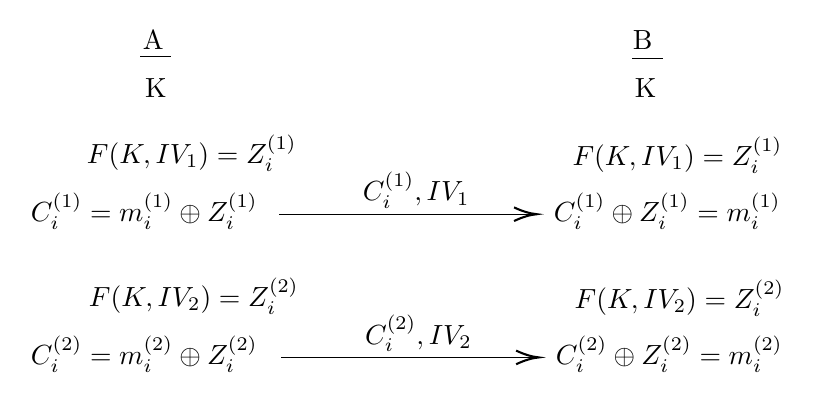
\begin{tikzpicture}[x=0.75pt,y=0.75pt,yscale=-1,xscale=1] 
            \draw    (139,71.6) -- (154,71.6) ;
            \draw    (376,72.6) -- (391,72.6) ;
            \draw    (206,147.6) -- (328,147.6) ;
            \draw [shift={(330,147.6)}, rotate = 180] [color={rgb, 255:red, 0; green, 0; blue, 0 }  ][line width=0.75]    (10.93,-3.29) .. controls (6.95,-1.4) and (3.31,-0.3) .. (0,0) .. controls (3.31,0.3) and (6.95,1.4) .. (10.93,3.29)   ;
            \draw    (207,216.6) -- (329,216.6) ;
            \draw [shift={(331,216.6)}, rotate = 180] [color={rgb, 255:red, 0; green, 0; blue, 0 }  ][line width=0.75]    (10.93,-3.29) .. controls (6.95,-1.4) and (3.31,-0.3) .. (0,0) .. controls (3.31,0.3) and (6.95,1.4) .. (10.93,3.29)   ;
            
            \draw (139,58) node [anchor=north west][inner sep=0.75pt]   [align=left] {A};
            \draw (375,58) node [anchor=north west][inner sep=0.75pt]   [align=left] {B};
            \draw (140,81) node [anchor=north west][inner sep=0.75pt]   [align=left] {K};
            \draw (376,81) node [anchor=north west][inner sep=0.75pt]   [align=left] {K};
            \draw (112,108) node [anchor=north west][inner sep=0.75pt]   [align=left] {$F(K,IV_1) = Z_i^{(1)}$};
            \draw (346,109) node [anchor=north west][inner sep=0.75pt]   [align=left] {$F(K,IV_1) = Z_i^{(1)}$};
            \draw (85,136) node [anchor=north west][inner sep=0.75pt]   [align=left] {$C_i^{(1)} = m_i^{(1)} \oplus Z_i^{(1)}$};
            \draw (337,136) node [anchor=north west][inner sep=0.75pt]   [align=left] {$C_i^{(1)} \oplus Z_i^{(1)} = m_i^{(1)}$};
            \draw (245,126) node [anchor=north west][inner sep=0.75pt]   [align=left] {$C_i^{(1)}, IV_1$};
            \draw (113,177) node [anchor=north west][inner sep=0.75pt]   [align=left] {$F(K,IV_2) = Z_i^{(2)}$};
            \draw (347,178) node [anchor=north west][inner sep=0.75pt]   [align=left] {$F(K,IV_2) = Z_i^{(2)}$};
            \draw (85,205) node [anchor=north west][inner sep=0.75pt]   [align=left] {$C_i^{(2)} = m_i^{(2)} \oplus Z_i^{(2)}$};
            \draw (338,205) node [anchor=north west][inner sep=0.75pt]   [align=left] {$C_i^{(2)} \oplus Z_i^{(2)} = m_i^{(2)}$};
            \draw (246,195) node [anchor=north west][inner sep=0.75pt]   [align=left] {$C_i^{(2)}, IV_2$};
        \end{tikzpicture}
    \end{center}    
\end{enumerate}
Hence, the advantages of this technique are that very long messages can be encrypted using a small key and the same key can be used to encrypt different messages.


\section{Stream Cipher}
A stream cipher consists of two things, a pseudo random bit generator and an encryption and decryption technique. The PBGR takes few inputs and generates keystream bits $Z_i$.
\begin{center}
    \textbf{PBGR:} $F(K,....) = Z_i$ (keystream bits)\\
    \textbf{Encryption:} $C_i = m_i \oplus Z_i$\\
    \textbf{Decryption:} $m_i = C_i \oplus Z_i$\\
\end{center}
We are using XOR here as as encryption technique, however it can be any other efficient computation too.

\subsection{Synchronous Stream Cipher}
A synchronous stream cipher is one in which the key stream is generated independently of plaintext and ciphertext bits. It has the following functions:
\begin{itemize}
    \item State Update function $\implies S_{i+1} = f(S_i, K)$\\
    \item Keystream Generator function $\implies Z_i = g(S_i, K)$\\
    \item Ciphertext Generation Function $\implies C_i = h(Z_i, m_i)$
\end{itemize}
Here $S_0$ is initial state and may be determined from K and IV. In synchronous stream cipher the functions $f$ and $g$ does not take plaintext and ciphertext input.

\subsection{Asynchronous or Self-Synchronizing Stream Ciphers}
An asynchronous stream cipher is one in which the keystream bits are generated as a function of key and a fixed number of previous cipher text bits.
\begin{itemize}
    \item State Update Function: $\sigma_{i+1} = f(\sigma, K, IV)$ where $\sigma = (C_{i-t}, C_{i - t + 1},....., C_{i-1})$\\
    \item Keystream Generation Function: $Z_i = g(\sigma_{i}, K)$\\
    \item Ciphertext Generation Function: $C_i = h(Z_i, m_i)$
\end{itemize}
Here, $\sigma_0 = (C_{-t}, C_{-t + 1},....., C_{-1})$ is the non-secret initial state.

\subsection{Linear Feedback Shift Register}
This is one of the most used stream cipher and has been used for every communication (voice calls) till 4G. It contains a n-bit register. The states are denoted by S, and the bits are denoted by s. There is a clock and at each clocking number the state of the register updates and the, an output (keystream bit) is generated using which encryption of message can be done.\\
A register of length n means that it is a n-bit LFSR, or equivalently it has a state of length n.\\
Let us say at clocking number t = 0, the state of the register is $S_0$. For each $0 \leq i \leq n-1$, $s_i \in \{0, 1\}$.
\begin{center}
    \tikzset{every picture/.style={line width=0.75pt}} 

    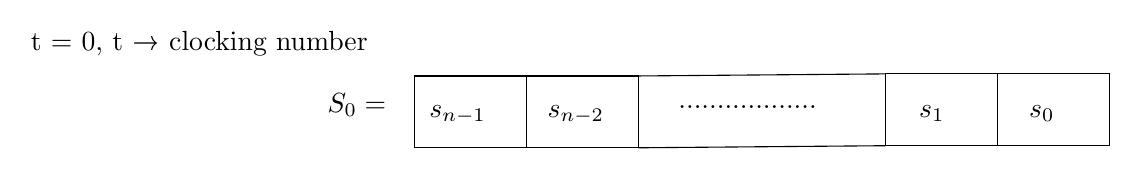
\begin{tikzpicture}[x=0.75pt,y=0.75pt,yscale=-1,xscale=1]
        \draw   (208,107) -- (262,107) -- (262,141.6) -- (208,141.6) -- cycle ; 
        \draw   (262,107) -- (316,107) -- (316,141.6) -- (262,141.6) -- cycle ;
        \draw   (435,106) -- (489,106) -- (489,140.6) -- (435,140.6) -- cycle ;
        \draw    (316,107) -- (435,106) ;
        \draw   (489,106) -- (543,106) -- (543,140.6) -- (489,140.6) -- cycle ;
        \draw    (316,141.6) -- (435,140.6) ;
        
        \draw (214,120) node [anchor=north west][inner sep=0.75pt]   [align=left] {$s_{n-1}$};
        \draw (271,120) node [anchor=north west][inner sep=0.75pt]   [align=left] {$s_{n-2}$};
        \draw (334,120) node [anchor=north west][inner sep=0.75pt]   [align=left] {..................};
        \draw (450,120) node [anchor=north west][inner sep=0.75pt]   [align=left] {$s_1$};
        \draw (503,120) node [anchor=north west][inner sep=0.75pt]   [align=left] {$s_0$};
        \draw (22,84) node [anchor=north west][inner sep=0.75pt]   [align=left] {t = 0, t → clocking number};
        \draw (165,114) node [anchor=north west][inner sep=0.75pt]   [align=left] {$S_0 = $};
    \end{tikzpicture}
\end{center}
At each clocking number, a shift by one bit takes place (either right or left, depends on the design). Here, we will take right shift for understanding.

\begin{center}
    \tikzset{every picture/.style={line width=0.75pt}} 
    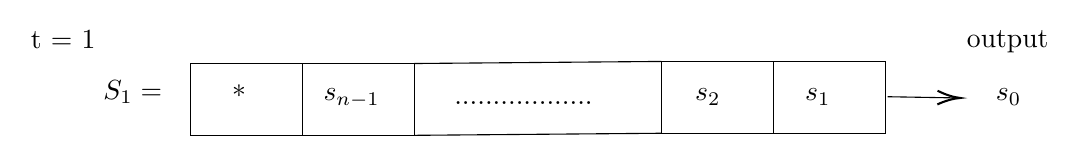
\begin{tikzpicture}[x=0.75pt,y=0.75pt,yscale=-1,xscale=1]
        \draw   (135,197) -- (189,197) -- (189,231.6) -- (135,231.6) -- cycle ;
        \draw   (189,197) -- (243,197) -- (243,231.6) -- (189,231.6) -- cycle ; 
        \draw   (362,196) -- (416,196) -- (416,230.6) -- (362,230.6) -- cycle ;
        \draw    (243,197) -- (362,196) ;
        \draw   (416,196) -- (470,196) -- (470,230.6) -- (416,230.6) -- cycle ;
        \draw    (243,231.6) -- (362,230.6) ;
        \draw    (471,213) -- (504,213.57) ;
        \draw [shift={(506,213.6)}, rotate = 180.98] [color={rgb, 255:red, 0; green, 0; blue, 0 }  ][line width=0.75]    (10.93,-3.29) .. controls (6.95,-1.4) and (3.31,-0.3) .. (0,0) .. controls (3.31,0.3) and (6.95,1.4) .. (10.93,3.29)   ;
        
        \draw (154,206) node [anchor=north west][inner sep=0.75pt]   [align=left] {*};
        \draw (198,208) node [anchor=north west][inner sep=0.75pt]   [align=left] {$s_{n-1}$};
        \draw (261,214) node [anchor=north west][inner sep=0.75pt]   [align=left] {..................};
        \draw (377,208) node [anchor=north west][inner sep=0.75pt]   [align=left] {$s_2$};
        \draw (430,208) node [anchor=north west][inner sep=0.75pt]   [align=left] {$s_1$};
        \draw (57,180) node [anchor=north west][inner sep=0.75pt]   [align=left] {t = 1};
        \draw (92,204) node [anchor=north west][inner sep=0.75pt]   [align=left] {$S_1 =$};
        \draw (508,180) node [anchor=north west][inner sep=0.75pt]   [align=left] {output};
        \draw (522,208) node [anchor=north west][inner sep=0.75pt]   [align=left] {$s_0$};
        
    \end{tikzpicture}
\end{center}

The rightmost bit $s_0$ moves out and is the output (the keystream bit). However, the leftmost bit $s_n$ becomes empty. $s_n$ is known as feedback bit and is calculated as:
\begin{center}
    $s_n = L(s_0, s_1,....., s_{n-1}) = L(S_0)$ 
\end{center}
After one more clocking, the state can be represented as:

\begin{center}
    \tikzset{every picture/.style={line width=0.75pt}} 
    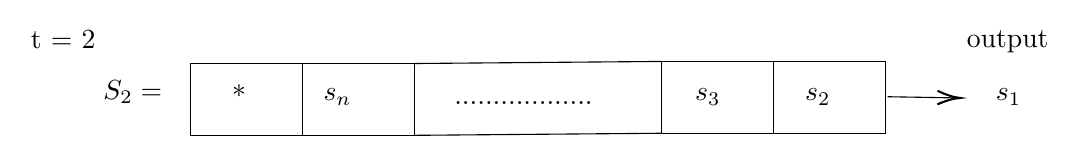
\begin{tikzpicture}[x=0.75pt,y=0.75pt,yscale=-1,xscale=1]
        \draw   (135,197) -- (189,197) -- (189,231.6) -- (135,231.6) -- cycle ;
        \draw   (189,197) -- (243,197) -- (243,231.6) -- (189,231.6) -- cycle ; 
        \draw   (362,196) -- (416,196) -- (416,230.6) -- (362,230.6) -- cycle ;
        \draw    (243,197) -- (362,196) ;
        \draw   (416,196) -- (470,196) -- (470,230.6) -- (416,230.6) -- cycle ;
        \draw    (243,231.6) -- (362,230.6) ;
        \draw    (471,213) -- (504,213.57) ;
        \draw [shift={(506,213.6)}, rotate = 180.98] [color={rgb, 255:red, 0; green, 0; blue, 0 }  ][line width=0.75]    (10.93,-3.29) .. controls (6.95,-1.4) and (3.31,-0.3) .. (0,0) .. controls (3.31,0.3) and (6.95,1.4) .. (10.93,3.29)   ;
        
        \draw (154,206) node [anchor=north west][inner sep=0.75pt]   [align=left] {*};
        \draw (198,208) node [anchor=north west][inner sep=0.75pt]   [align=left] {$s_n$};
        \draw (261,214) node [anchor=north west][inner sep=0.75pt]   [align=left] {..................};
        \draw (377,208) node [anchor=north west][inner sep=0.75pt]   [align=left] {$s_3$};
        \draw (430,208) node [anchor=north west][inner sep=0.75pt]   [align=left] {$s_2$};
        \draw (57,180) node [anchor=north west][inner sep=0.75pt]   [align=left] {t = 2};
        \draw (92,204) node [anchor=north west][inner sep=0.75pt]   [align=left] {$S_2 =$};
        \draw (508,180) node [anchor=north west][inner sep=0.75pt]   [align=left] {output};
        \draw (522,208) node [anchor=north west][inner sep=0.75pt]   [align=left] {$s_1$};
        
    \end{tikzpicture}
\end{center}
Again, the feedback bit $S_{n+1} = L(S_1)$. We will look at the function L in some time. The LFSR with right shift operation can be represented with the following circuit.
\begin{center}
    \tikzset{every picture/.style={line width=0.75pt}} 
    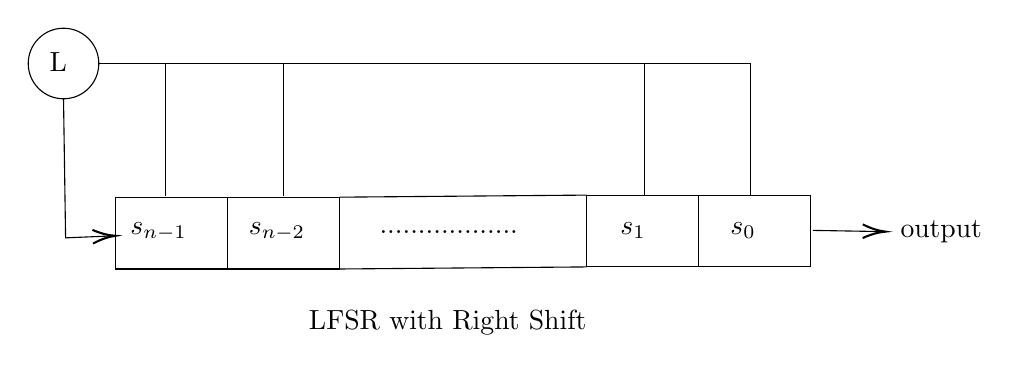
\begin{tikzpicture}[x=0.75pt,y=0.75pt,yscale=-1,xscale=1]
        \draw   (138,147) -- (192,147) -- (192,181.6) -- (138,181.6) -- cycle ;
        \draw   (192,147) -- (246,147) -- (246,181.6) -- (192,181.6) -- cycle ;
        \draw   (365,146) -- (419,146) -- (419,180.6) -- (365,180.6) -- cycle ; 
        \draw    (246,147) -- (365,146) ;
        \draw   (419,146) -- (473,146) -- (473,180.6) -- (419,180.6) -- cycle ;
        \draw    (246,181.6) -- (365,180.6) ; 
        \draw    (474,163) -- (507,163.57) ;
        \draw [shift={(509,163.6)}, rotate = 180.98] [color={rgb, 255:red, 0; green, 0; blue, 0 }  ][line width=0.75]    (10.93,-3.29) .. controls (6.95,-1.4) and (3.31,-0.3) .. (0,0) .. controls (3.31,0.3) and (6.95,1.4) .. (10.93,3.29)   ;
        \draw    (130,82.6) -- (444,82.6) -- (444,146) ;
        \draw   (96,82.6) .. controls (96,73.21) and (103.61,65.6) .. (113,65.6) .. controls (122.39,65.6) and (130,73.21) .. (130,82.6) .. controls (130,91.99) and (122.39,99.6) .. (113,99.6) .. controls (103.61,99.6) and (96,91.99) .. (96,82.6) -- cycle ;
        \draw    (113,99.6) -- (114,166.6) -- (136,165.68) ;
        \draw [shift={(138,165.6)}, rotate = 177.61] [color={rgb, 255:red, 0; green, 0; blue, 0 }  ][line width=0.75]    (10.93,-3.29) .. controls (6.95,-1.4) and (3.31,-0.3) .. (0,0) .. controls (3.31,0.3) and (6.95,1.4) .. (10.93,3.29)   ;
        \draw    (162,82.6) -- (162,146.6) ;
        \draw    (219,82.6) -- (219,146.6) ;
        \draw    (393,82.6) -- (393,146.6) ;
        
        \draw (144,158) node [anchor=north west][inner sep=0.75pt]   [align=left] {$s_{n-1}$};
        \draw (201,158) node [anchor=north west][inner sep=0.75pt]   [align=left] {$s_{n-2}$};
        \draw (264,162) node [anchor=north west][inner sep=0.75pt]   [align=left] {..................};
        \draw (380,158) node [anchor=north west][inner sep=0.75pt]   [align=left] {$s_1$};
        \draw (433,158) node [anchor=north west][inner sep=0.75pt]   [align=left] {$s_0$};
        \draw (515,157) node [anchor=north west][inner sep=0.75pt]   [align=left] {output};
        \draw (105,76) node [anchor=north west][inner sep=0.75pt]   [align=left] {L};
        \draw (230,200) node [anchor=north west][inner sep=0.75pt]   [align=left] {LFSR with Right Shift};
    \end{tikzpicture}
\end{center}

The function L is a linear function on the bits of the previous state.
\begin{center}
    $L: \{0,1\}^n \rightarrow \{0,1\}$\\
    $L(s_0, s_1,....., s_{n-1}) = s_n$
\end{center}
A linear function can be represented as:
\begin{center}
    $L_a = a_0\cdot s_0 \oplus a_1 \cdot s_1 \oplus ..... \oplus a_{n-1} \cdot s_{n-1}$ where $a_i \in \{0, 1\}$
\end{center}

Suppose, an arbitrary function L be defined as:
\begin{center}
    $L = a_0\cdot s_0 \oplus a_1 \cdot s_1 \oplus ..... \oplus a_{n-1} \cdot s_{n-1} \oplus a_n$ where $a_i \in \{0, 1\}$
\end{center}
In this function, if $a_n = 0$ then $L = L_a$, a linear function. Otherwise, if $a_n = 1$ the $L \neq L_a$. In fact, such a function is known as Affine function.

A function can be proved to be linear using the following property.
\begin{center}
    $L(X) \oplus L(Y) = L(X \oplus Y)$\\
    $\implies L(X) \oplus L(Y) \oplus L(X \oplus Y) = 0$
\end{center}
\textbf{Example:} Find if the following functions are linear or not. Solve it considering 2-bit inputs.
\begin{enumerate}
    \item $L_1(x, y) = x \oplus y$
    \item $L_2(x, y) = 1 \oplus x \oplus y$

\end{enumerate}
\textbf{Solution:} 
\begin{enumerate}
    \item Let's compute $L_1(x) \oplus L_1(y) \oplus L_1(x \oplus y)$
    \begin{center}
        $L_1(x) \oplus L_1(y) \oplus L_1(x \oplus y) = (x_1 \oplus x_2) \oplus (y_1 \oplus y_2) \oplus ((x_1 \oplus y_1) \oplus (x_2 \oplus y_2))$\\
        \vspace{1mm}
        $L_1(x) \oplus L_1(y) \oplus L_1(x \oplus y) = 0$
    \end{center}
    Therefore, $L_1$ is a linear function.
    \item $L_2(x) \oplus L_2(y) \oplus L_2(x \oplus y) = (1 \oplus x_1 \oplus x_2) \oplus (1 \oplus y_1 \oplus y_2) \oplus (1 \oplus (x_1 \oplus y_1) \oplus (x_2 \oplus y_2))$
    \begin{center}
        $L_2(x) \oplus L_2(y) \oplus L_2(x \oplus y) = 1 $
    \end{center}
    Therefore, $L_2$ is not a linear function.
\end{enumerate}

LFSR has a linear function, whose output depends on previous state, therefore it provides feedback. There is shift operation on the bits stored in register. Hence, the name is Linear Feedback Shift Register. \\
Now, let us see an example of a 3-bit LFSR.

\begin{center}
    \tikzset{every picture/.style={line width=0.75pt}}
    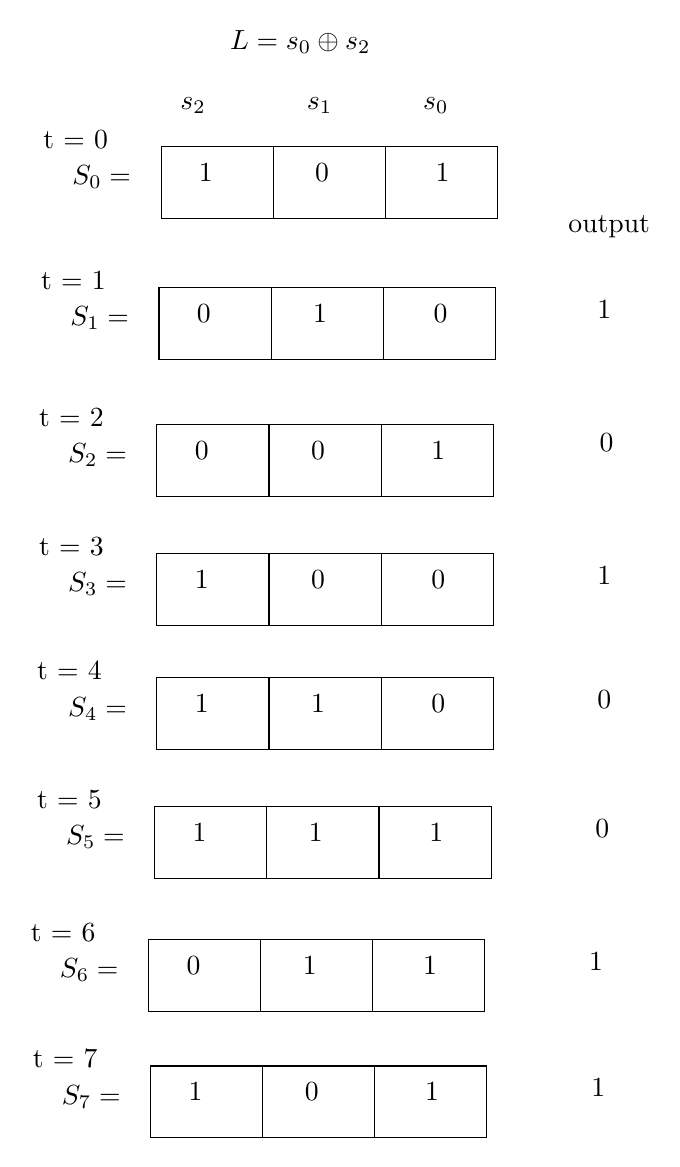
\begin{tikzpicture}[x=0.75pt,y=0.75pt,yscale=-1,xscale=1]
        
        \draw   (230,277) -- (284,277) -- (284,311.6) -- (230,311.6) -- cycle ;
        \draw   (284,277) -- (338,277) -- (338,311.6) -- (284,311.6) -- cycle ;
        \draw   (338,277) -- (392,277) -- (392,311.6) -- (338,311.6) -- cycle ;
        \draw   (229,345) -- (283,345) -- (283,379.6) -- (229,379.6) -- cycle ;
        \draw   (283,345) -- (337,345) -- (337,379.6) -- (283,379.6) -- cycle ;
        \draw   (337,345) -- (391,345) -- (391,379.6) -- (337,379.6) -- cycle ;
        \draw   (228,411) -- (282,411) -- (282,445.6) -- (228,445.6) -- cycle ;
        \draw   (282,411) -- (336,411) -- (336,445.6) -- (282,445.6) -- cycle ;
        \draw   (336,411) -- (390,411) -- (390,445.6) -- (336,445.6) -- cycle ;
        \draw   (228,473) -- (282,473) -- (282,507.6) -- (228,507.6) -- cycle ;
        \draw   (282,473) -- (336,473) -- (336,507.6) -- (282,507.6) -- cycle ;
        \draw   (336,473) -- (390,473) -- (390,507.6) -- (336,507.6) -- cycle ;
        \draw   (228,533) -- (282,533) -- (282,567.6) -- (228,567.6) -- cycle ;
        \draw   (282,533) -- (336,533) -- (336,567.6) -- (282,567.6) -- cycle ;
        \draw   (336,533) -- (390,533) -- (390,567.6) -- (336,567.6) -- cycle ;
        \draw   (227,595) -- (281,595) -- (281,629.6) -- (227,629.6) -- cycle ;
        \draw   (281,595) -- (335,595) -- (335,629.6) -- (281,629.6) -- cycle ;
        \draw   (335,595) -- (389,595) -- (389,629.6) -- (335,629.6) -- cycle ;
        \draw   (224,659) -- (278,659) -- (278,693.6) -- (224,693.6) -- cycle ;
        \draw   (278,659) -- (332,659) -- (332,693.6) -- (278,693.6) -- cycle ;
        \draw   (332,659) -- (386,659) -- (386,693.6) -- (332,693.6) -- cycle ;
        \draw   (225,720) -- (279,720) -- (279,754.6) -- (225,754.6) -- cycle ;
        \draw   (279,720) -- (333,720) -- (333,754.6) -- (279,754.6) -- cycle ;
        \draw   (333,720) -- (387,720) -- (387,754.6) -- (333,754.6) -- cycle ;
        
        \draw (303,284) node [anchor=north west][inner sep=0.75pt]   [align=left] {0};
        \draw (262,220) node [anchor=north west][inner sep=0.75pt]   [align=left] {$L = s_0 \oplus s_2$};
        \draw (238,252) node [anchor=north west][inner sep=0.75pt]   [align=left] {$s_2$};
        \draw (299,252) node [anchor=north west][inner sep=0.75pt]   [align=left] {$s_1$};
        \draw (355,252) node [anchor=north west][inner sep=0.75pt]   [align=left] {$s_0$};
        \draw (172,268) node [anchor=north west][inner sep=0.75pt]   [align=left] {t = 0};
        \draw (186,285) node [anchor=north west][inner sep=0.75pt]   [align=left] {$S_0 = $};
        \draw (425,309) node [anchor=north west][inner sep=0.75pt]   [align=left] {output};
        \draw (247,284) node [anchor=north west][inner sep=0.75pt]   [align=left] {1};
        \draw (361,284) node [anchor=north west][inner sep=0.75pt]   [align=left] {1};
        \draw (302,352) node [anchor=north west][inner sep=0.75pt]   [align=left] {1};
        \draw (171,336) node [anchor=north west][inner sep=0.75pt]   [align=left] {t = 1};
        \draw (185,353) node [anchor=north west][inner sep=0.75pt]   [align=left] {$S_1 = $};
        \draw (246,352) node [anchor=north west][inner sep=0.75pt]   [align=left] {0};
        \draw (360,352) node [anchor=north west][inner sep=0.75pt]   [align=left] {0};
        \draw (301,418) node [anchor=north west][inner sep=0.75pt]   [align=left] {0};
        \draw (170,402) node [anchor=north west][inner sep=0.75pt]   [align=left] {t = 2};
        \draw (184,419) node [anchor=north west][inner sep=0.75pt]   [align=left] {$S_2 = $};
        \draw (245,418) node [anchor=north west][inner sep=0.75pt]   [align=left] {0};
        \draw (359,418) node [anchor=north west][inner sep=0.75pt]   [align=left] {1};
        \draw (301,480) node [anchor=north west][inner sep=0.75pt]   [align=left] {0};
        \draw (170,464) node [anchor=north west][inner sep=0.75pt]   [align=left] {t = 3};
        \draw (184,481) node [anchor=north west][inner sep=0.75pt]   [align=left] {$S_3 = $};
        \draw (245,480) node [anchor=north west][inner sep=0.75pt]   [align=left] {1};
        \draw (359,480) node [anchor=north west][inner sep=0.75pt]   [align=left] {0};
        \draw (439,350) node [anchor=north west][inner sep=0.75pt]   [align=left] {1};
        \draw (440,414) node [anchor=north west][inner sep=0.75pt]   [align=left] {0};
        \draw (439,478) node [anchor=north west][inner sep=0.75pt]   [align=left] {1};
        \draw (301,540) node [anchor=north west][inner sep=0.75pt]   [align=left] {1};
        \draw (169,524) node [anchor=north west][inner sep=0.75pt]   [align=left] {t = 4};
        \draw (184,541) node [anchor=north west][inner sep=0.75pt]   [align=left] {$S_4 = $};
        \draw (245,540) node [anchor=north west][inner sep=0.75pt]   [align=left] {1};
        \draw (359,540) node [anchor=north west][inner sep=0.75pt]   [align=left] {0};
        \draw (439,538) node [anchor=north west][inner sep=0.75pt]   [align=left] {0};
        \draw (300,602) node [anchor=north west][inner sep=0.75pt]   [align=left] {1};
        \draw (169,586) node [anchor=north west][inner sep=0.75pt]   [align=left] {t = 5};
        \draw (183,603) node [anchor=north west][inner sep=0.75pt]   [align=left] {$S_5 = $};
        \draw (244,602) node [anchor=north west][inner sep=0.75pt]   [align=left] {1};
        \draw (358,602) node [anchor=north west][inner sep=0.75pt]   [align=left] {1};
        \draw (438,600) node [anchor=north west][inner sep=0.75pt]   [align=left] {0};
        \draw (297,666) node [anchor=north west][inner sep=0.75pt]   [align=left] {1};
        \draw (166,650) node [anchor=north west][inner sep=0.75pt]   [align=left] {t = 6};
        \draw (180,667) node [anchor=north west][inner sep=0.75pt]   [align=left] {$S_6 = $};
        \draw (241,666) node [anchor=north west][inner sep=0.75pt]   [align=left] {0};
        \draw (355,666) node [anchor=north west][inner sep=0.75pt]   [align=left] {1};
        \draw (435,664) node [anchor=north west][inner sep=0.75pt]   [align=left] {1};
        \draw (298,727) node [anchor=north west][inner sep=0.75pt]   [align=left] {0};
        \draw (167,711) node [anchor=north west][inner sep=0.75pt]   [align=left] {t = 7};
        \draw (181,728) node [anchor=north west][inner sep=0.75pt]   [align=left] {$S_7 = $};
        \draw (242,727) node [anchor=north west][inner sep=0.75pt]   [align=left] {1};
        \draw (356,727) node [anchor=north west][inner sep=0.75pt]   [align=left] {1};
        \draw (436,725) node [anchor=north west][inner sep=0.75pt]   [align=left] {1};        
    \end{tikzpicture}
\end{center}

The L function for this LFSR is $L = s_0 \oplus s_2$.\\
In any LFSR, if you have reached the initial state again, the the output bits will be repeated. In the above example it can be seen that from start state t = 0 to the state t = 7, all the non-zero states are obtained.\\
The output bits in the above example are repeated after $t = 2^3 - 1$ states because at t = 7, the initial state is reached. Hence, maximum output length that can be achieved in this LFSR without repetition is 7.
Hence, using LFSR, only $2^n - 1$ maximum number of non-zero states can be generated.\\
Also, if we take the 0 state i.e. all bits in the register are 0, it will remain in the zero state forever. Hence, in any LFSR, if input state is 0, then it will remain zero. Hence, LFSR has a fixed point (0-state).\\

Let us look at another example of a 3-bit LFSR with a different L function. This time the L function is $L = s_0$.

\begin{center}   
    \tikzset{every picture/.style={line width=0.75pt}}
    \begin{tikzpicture}[x=0.75pt,y=0.75pt,yscale=-1,xscale=1]
        \draw   (230,277) -- (284,277) -- (284,311.6) -- (230,311.6) -- cycle ;
        \draw   (284,277) -- (338,277) -- (338,311.6) -- (284,311.6) -- cycle ; 
        \draw   (338,277) -- (392,277) -- (392,311.6) -- (338,311.6) -- cycle ; 
        \draw   (229,345) -- (283,345) -- (283,379.6) -- (229,379.6) -- cycle ;
        \draw   (283,345) -- (337,345) -- (337,379.6) -- (283,379.6) -- cycle ;
        \draw   (337,345) -- (391,345) -- (391,379.6) -- (337,379.6) -- cycle ;
        \draw   (228,411) -- (282,411) -- (282,445.6) -- (228,445.6) -- cycle ;
        \draw   (282,411) -- (336,411) -- (336,445.6) -- (282,445.6) -- cycle ;
        \draw   (336,411) -- (390,411) -- (390,445.6) -- (336,445.6) -- cycle ;
        \draw   (228,473) -- (282,473) -- (282,507.6) -- (228,507.6) -- cycle ;
        \draw   (282,473) -- (336,473) -- (336,507.6) -- (282,507.6) -- cycle ;
        \draw   (336,473) -- (390,473) -- (390,507.6) -- (336,507.6) -- cycle ;
        
        
        \draw (303,284) node [anchor=north west][inner sep=0.75pt]   [align=left] {0};
        \draw (290,220) node [anchor=north west][inner sep=0.75pt]   [align=left] {$L = s0$};
        \draw (238,252) node [anchor=north west][inner sep=0.75pt]   [align=left] {$s_2$};
        \draw (299,252) node [anchor=north west][inner sep=0.75pt]   [align=left] {$s_1$};
        \draw (355,252) node [anchor=north west][inner sep=0.75pt]   [align=left] {$s_0$};
        \draw (172,268) node [anchor=north west][inner sep=0.75pt]   [align=left] {t = 0};
        \draw (186,285) node [anchor=north west][inner sep=0.75pt]   [align=left] {$S_0 = $};
        \draw (425,309) node [anchor=north west][inner sep=0.75pt]   [align=left] {output};
        \draw (247,284) node [anchor=north west][inner sep=0.75pt]   [align=left] {1};
        \draw (361,284) node [anchor=north west][inner sep=0.75pt]   [align=left] {1};
        \draw (302,352) node [anchor=north west][inner sep=0.75pt]   [align=left] {1};
        \draw (171,336) node [anchor=north west][inner sep=0.75pt]   [align=left] {t = 1};
        \draw (185,353) node [anchor=north west][inner sep=0.75pt]   [align=left] {$S_1 = $};
        \draw (246,352) node [anchor=north west][inner sep=0.75pt]   [align=left] {1};
        \draw (360,352) node [anchor=north west][inner sep=0.75pt]   [align=left] {0};
        \draw (301,418) node [anchor=north west][inner sep=0.75pt]   [align=left] {1};
        \draw (170,402) node [anchor=north west][inner sep=0.75pt]   [align=left] {t = 2};
        \draw (184,419) node [anchor=north west][inner sep=0.75pt]   [align=left] {$S_2 = $};
        \draw (245,418) node [anchor=north west][inner sep=0.75pt]   [align=left] {0};
        \draw (359,418) node [anchor=north west][inner sep=0.75pt]   [align=left] {1};
        \draw (301,480) node [anchor=north west][inner sep=0.75pt]   [align=left] {0};
        \draw (170,464) node [anchor=north west][inner sep=0.75pt]   [align=left] {t = 3};
        \draw (184,481) node [anchor=north west][inner sep=0.75pt]   [align=left] {$S_3 = $};
        \draw (245,480) node [anchor=north west][inner sep=0.75pt]   [align=left] {1};
        \draw (359,480) node [anchor=north west][inner sep=0.75pt]   [align=left] {1};
        \draw (439,350) node [anchor=north west][inner sep=0.75pt]   [align=left] {1};
        \draw (440,414) node [anchor=north west][inner sep=0.75pt]   [align=left] {0};
        \draw (439,478) node [anchor=north west][inner sep=0.75pt]   [align=left] {1};        
    \end{tikzpicture}
\end{center}
Here, we can see the initial state is reached again only at t = 3. For LFSR, the linear functionis very important in deciding the period after which the bits will repeat.

\subsubsection{Period of an LFSR} 
Consider $S_0$ to be a non-zero state. $S_0$ is repeated after $m$ clocking of LFSR, then $m$ will be the period of LFSR. An LFSR with n-bits can have a maximum period of $2^n - 1$.\\


If there is an LFSR where different non-zero states are repeating at certain different number of clocking. Let us say $x_1$ number of states repeat after $P_1$ clocking, $x_2$ number of states repeat after $P_2$ clocking and so on $x_n$ number of states repeat after $P_N$ clocking. Here, every non-zero state is present in at least and only one $x_i$. Therefore, if we take any non-zero state, then it will repeat after certain number of clocking which will belong to the set $\{P_1, P_2,...., P_N\}$. Therefore, the period of LFSR will be:
\begin{center}
    Period of LFSR = $LCM(P_1, P_2,...., P_N)$
\end{center}
Consider an n-bit LFSR,
\begin{center}
    \tikzset{every picture/.style={line width=0.75pt}} 
    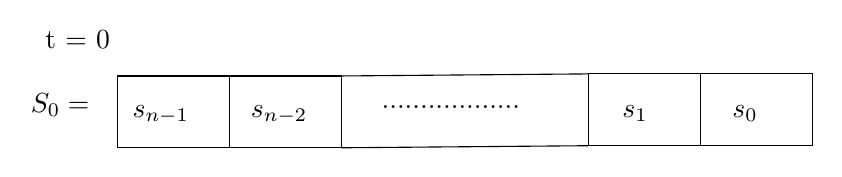
\begin{tikzpicture}[x=0.75pt,y=0.75pt,yscale=-1,xscale=1]
        \draw   (208,107) -- (262,107) -- (262,141.6) -- (208,141.6) -- cycle ; 
        \draw   (262,107) -- (316,107) -- (316,141.6) -- (262,141.6) -- cycle ;
        \draw   (435,106) -- (489,106) -- (489,140.6) -- (435,140.6) -- cycle ;
        \draw    (316,107) -- (435,106) ;
        \draw   (489,106) -- (543,106) -- (543,140.6) -- (489,140.6) -- cycle ;
        \draw    (316,141.6) -- (435,140.6) ;
        
        \draw (214,120) node [anchor=north west][inner sep=0.75pt]   [align=left] {$s_{n-1}$};
        \draw (271,120) node [anchor=north west][inner sep=0.75pt]   [align=left] {$s_{n-2}$};
        \draw (334,120) node [anchor=north west][inner sep=0.75pt]   [align=left] {..................};
        \draw (450,120) node [anchor=north west][inner sep=0.75pt]   [align=left] {$s_1$};
        \draw (503,120) node [anchor=north west][inner sep=0.75pt]   [align=left] {$s_0$};
        \draw (172,84) node [anchor=north west][inner sep=0.75pt]   [align=left] {t = 0};
        \draw (165,114) node [anchor=north west][inner sep=0.75pt]   [align=left] {$S_0 = $};
    \end{tikzpicture}
\end{center}
We know that after clocking, $s_n$ will be,
\begin{center}
    $s_n = L(s_0,s_1,...., s_{n-1})$\\
    $s_n = c_1\cdot s_{n-1} \oplus c_2 \cdot s_{n-2} \oplus ..... \oplus c_n \cdot s_0$ where $c_i \in \{0, 1\}$
\end{center}
This is known as Algebraic Normal Form of writing $s_n$. Therefore, we can see that to implement LFSR in hardware, we only need AND and XOR gates. The circuit for LFSR is given below. The value of $s_i$ will be xored or not depends on the value of $c_{n-i}$.

\begin{center}
    \tikzset{every picture/.style={line width=0.75pt}} 
    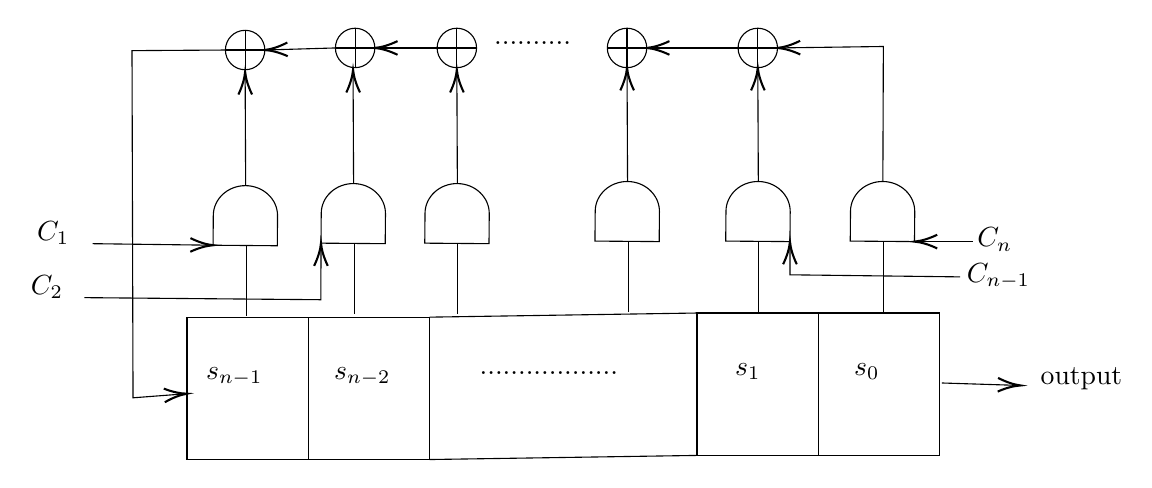
\begin{tikzpicture}[x=0.75pt,y=0.75pt,yscale=-1,xscale=1]
        \draw   (110.47,177.2) -- (168.93,177.2) -- (168.93,245.8) -- (110.47,245.8) -- cycle ;
        \draw   (168.93,177.2) -- (227.39,177.2) -- (227.39,245.8) -- (168.93,245.8) -- cycle ;
        \draw   (356.22,175.21) -- (414.68,175.21) -- (414.68,243.82) -- (356.22,243.82) -- cycle ; 
        \draw    (227.39,177.2) -- (356.22,175.21) ;
        \draw   (414.68,175.21) -- (473.14,175.21) -- (473.14,243.82) -- (414.68,243.82) -- cycle ;
        \draw    (227.39,245.8) -- (356.22,243.82) ;
        \draw    (474.22,208.92) -- (510.11,210.05) ;
        \draw [shift={(512.11,210.11)}, rotate = 181.8] [color={rgb, 255:red, 0; green, 0; blue, 0 }  ][line width=0.75]    (10.93,-3.29) .. controls (6.95,-1.4) and (3.31,-0.3) .. (0,0) .. controls (3.31,0.3) and (6.95,1.4) .. (10.93,3.29)   ;
        \draw    (129,48.5) -- (84,48.8) -- (84.49,216.06) -- (108.47,214.23) ;
        \draw [shift={(110.47,214.08)}, rotate = 175.64] [color={rgb, 255:red, 0; green, 0; blue, 0 }  ][line width=0.75]    (10.93,-3.29) .. controls (6.95,-1.4) and (3.31,-0.3) .. (0,0) .. controls (3.31,0.3) and (6.95,1.4) .. (10.93,3.29)   ;
        \draw   (370.05,140.55) -- (370.17,126.13) .. controls (370.24,118.17) and (377.22,111.77) .. (385.76,111.84) .. controls (394.31,111.91) and (401.18,118.42) .. (401.12,126.38) -- (401,140.8) -- cycle ;
        \draw    (386,140.8) -- (386,174.8) ; 
        \draw   (129,48.5) .. controls (129,43.25) and (133.25,39) .. (138.5,39) .. controls (143.75,39) and (148,43.25) .. (148,48.5) .. controls (148,53.75) and (143.75,58) .. (138.5,58) .. controls (133.25,58) and (129,53.75) .. (129,48.5) -- cycle ; \draw   (129,48.5) -- (148,48.5) ; \draw   (138.5,39) -- (138.5,58) ;
        \draw   (182,47.5) .. controls (182,42.25) and (186.25,38) .. (191.5,38) .. controls (196.75,38) and (201,42.25) .. (201,47.5) .. controls (201,52.75) and (196.75,57) .. (191.5,57) .. controls (186.25,57) and (182,52.75) .. (182,47.5) -- cycle ; \draw   (182,47.5) -- (201,47.5) ; \draw   (191.5,38) -- (191.5,57) ;
        \draw   (231,47.5) .. controls (231,42.25) and (235.25,38) .. (240.5,38) .. controls (245.75,38) and (250,42.25) .. (250,47.5) .. controls (250,52.75) and (245.75,57) .. (240.5,57) .. controls (235.25,57) and (231,52.75) .. (231,47.5) -- cycle ; \draw   (231,47.5) -- (250,47.5) ; \draw   (240.5,38) -- (240.5,57) ;
        \draw   (313,47.5) .. controls (313,42.25) and (317.25,38) .. (322.5,38) .. controls (327.75,38) and (332,42.25) .. (332,47.5) .. controls (332,52.75) and (327.75,57) .. (322.5,57) .. controls (317.25,57) and (313,52.75) .. (313,47.5) -- cycle ; \draw   (313,47.5) -- (332,47.5) ; \draw   (322.5,38) -- (322.5,57) ;
        \draw   (376,47.5) .. controls (376,42.25) and (380.25,38) .. (385.5,38) .. controls (390.75,38) and (395,42.25) .. (395,47.5) .. controls (395,52.75) and (390.75,57) .. (385.5,57) .. controls (380.25,57) and (376,52.75) .. (376,47.5) -- cycle ; \draw   (376,47.5) -- (395,47.5) ; \draw   (385.5,38) -- (385.5,57) ;
        \draw    (376,47.5) -- (334,47.5) ;
        \draw [shift={(332,47.5)}, rotate = 360] [color={rgb, 255:red, 0; green, 0; blue, 0 }  ][line width=0.75]    (10.93,-3.29) .. controls (6.95,-1.4) and (3.31,-0.3) .. (0,0) .. controls (3.31,0.3) and (6.95,1.4) .. (10.93,3.29)   ;
        \draw    (231,47.5) -- (203,47.5) ;
        \draw [shift={(201,47.5)}, rotate = 360] [color={rgb, 255:red, 0; green, 0; blue, 0 }  ][line width=0.75]    (10.93,-3.29) .. controls (6.95,-1.4) and (3.31,-0.3) .. (0,0) .. controls (3.31,0.3) and (6.95,1.4) .. (10.93,3.29)   ;
        \draw    (182,47.5) -- (150,48.44) ;
        \draw [shift={(148,48.5)}, rotate = 358.32] [color={rgb, 255:red, 0; green, 0; blue, 0 }  ][line width=0.75]    (10.93,-3.29) .. controls (6.95,-1.4) and (3.31,-0.3) .. (0,0) .. controls (3.31,0.3) and (6.95,1.4) .. (10.93,3.29)   ;
        \draw    (385.76,111.84) -- (385.51,59) ;
        \draw [shift={(385.5,57)}, rotate = 89.73] [color={rgb, 255:red, 0; green, 0; blue, 0 }  ][line width=0.75]    (10.93,-3.29) .. controls (6.95,-1.4) and (3.31,-0.3) .. (0,0) .. controls (3.31,0.3) and (6.95,1.4) .. (10.93,3.29)   ;
        \draw   (307.05,140.55) -- (307.17,126.13) .. controls (307.24,118.17) and (314.22,111.77) .. (322.76,111.84) .. controls (331.31,111.91) and (338.18,118.42) .. (338.12,126.38) -- (338,140.8) -- cycle ;
        \draw    (323,140.8) -- (323,174.8) ;
        \draw    (322.76,111.84) -- (322.51,59) ;
        \draw [shift={(322.5,57)}, rotate = 89.73] [color={rgb, 255:red, 0; green, 0; blue, 0 }  ][line width=0.75]    (10.93,-3.29) .. controls (6.95,-1.4) and (3.31,-0.3) .. (0,0) .. controls (3.31,0.3) and (6.95,1.4) .. (10.93,3.29)   ;
        \draw   (225.05,141.55) -- (225.17,127.13) .. controls (225.24,119.17) and (232.22,112.77) .. (240.76,112.84) .. controls (249.31,112.91) and (256.18,119.42) .. (256.12,127.38) -- (256,141.8) -- cycle ;
        \draw    (241,141.8) -- (241,175.8) ; 
        \draw    (240.76,112.84) -- (240.51,60) ;
        \draw [shift={(240.5,58)}, rotate = 89.73] [color={rgb, 255:red, 0; green, 0; blue, 0 }  ][line width=0.75]    (10.93,-3.29) .. controls (6.95,-1.4) and (3.31,-0.3) .. (0,0) .. controls (3.31,0.3) and (6.95,1.4) .. (10.93,3.29)   ;
        \draw   (175.05,141.55) -- (175.17,127.13) .. controls (175.24,119.17) and (182.22,112.77) .. (190.76,112.84) .. controls (199.31,112.91) and (206.18,119.42) .. (206.12,127.38) -- (206,141.8) -- cycle ;
        \draw    (191,141.8) -- (191,175.8) ; 
        \draw    (190.76,112.84) -- (190.51,60) ;
        \draw [shift={(190.5,58)}, rotate = 89.73] [color={rgb, 255:red, 0; green, 0; blue, 0 }  ][line width=0.75]    (10.93,-3.29) .. controls (6.95,-1.4) and (3.31,-0.3) .. (0,0) .. controls (3.31,0.3) and (6.95,1.4) .. (10.93,3.29)   ; 
        \draw   (123.05,142.55) -- (123.17,128.13) .. controls (123.24,120.17) and (130.22,113.77) .. (138.76,113.84) .. controls (147.31,113.91) and (154.18,120.42) .. (154.12,128.38) -- (154,142.8) -- cycle ;
        \draw    (139,142.8) -- (139,176.8) ;
        \draw    (138.76,113.84) -- (138.51,61) ;
        \draw [shift={(138.5,59)}, rotate = 89.73] [color={rgb, 255:red, 0; green, 0; blue, 0 }  ][line width=0.75]    (10.93,-3.29) .. controls (6.95,-1.4) and (3.31,-0.3) .. (0,0) .. controls (3.31,0.3) and (6.95,1.4) .. (10.93,3.29)   ;
        \draw   (430.05,140.55) -- (430.17,126.13) .. controls (430.24,118.17) and (437.22,111.77) .. (445.76,111.84) .. controls (454.31,111.91) and (461.18,118.42) .. (461.12,126.38) -- (461,140.8) -- cycle ;
        \draw    (446,140.8) -- (446,174.8) ;
        \draw    (445.76,111.84) -- (446,46.8) -- (397,47.47) ;
        \draw [shift={(395,47.5)}, rotate = 359.21] [color={rgb, 255:red, 0; green, 0; blue, 0 }  ][line width=0.75]    (10.93,-3.29) .. controls (6.95,-1.4) and (3.31,-0.3) .. (0,0) .. controls (3.31,0.3) and (6.95,1.4) .. (10.93,3.29)   ;
        \draw    (489,140.8) -- (463,140.8) ;
        \draw [shift={(461,140.8)}, rotate = 360] [color={rgb, 255:red, 0; green, 0; blue, 0 }  ][line width=0.75]    (10.93,-3.29) .. controls (6.95,-1.4) and (3.31,-0.3) .. (0,0) .. controls (3.31,0.3) and (6.95,1.4) .. (10.93,3.29)   ;
        \draw    (483,157.8) -- (401,156.8) -- (401,142.8) ;
        \draw [shift={(401,140.8)}, rotate = 90] [color={rgb, 255:red, 0; green, 0; blue, 0 }  ][line width=0.75]    (10.93,-3.29) .. controls (6.95,-1.4) and (3.31,-0.3) .. (0,0) .. controls (3.31,0.3) and (6.95,1.4) .. (10.93,3.29)   ;
        \draw    (61,167.8) -- (175,168.8) -- (175.05,143.55) ;
        \draw [shift={(175.05,141.55)}, rotate = 90.11] [color={rgb, 255:red, 0; green, 0; blue, 0 }  ][line width=0.75]    (10.93,-3.29) .. controls (6.95,-1.4) and (3.31,-0.3) .. (0,0) .. controls (3.31,0.3) and (6.95,1.4) .. (10.93,3.29)   ;
        \draw    (65,141.8) -- (121.05,142.52) ;
        \draw [shift={(123.05,142.55)}, rotate = 180.74] [color={rgb, 255:red, 0; green, 0; blue, 0 }  ][line width=0.75]    (10.93,-3.29) .. controls (6.95,-1.4) and (3.31,-0.3) .. (0,0) .. controls (3.31,0.3) and (6.95,1.4) .. (10.93,3.29)   ;
        
        \draw (118.41,200.39) node [anchor=north west][inner sep=0.75pt]   [align=left] {$s_{n-1}$};
        \draw (180.12,200.39) node [anchor=north west][inner sep=0.75pt]   [align=left] {$s_{n-2}$};
        \draw (250.22,202.38) node [anchor=north west][inner sep=0.75pt]   [align=left] {..................};
        \draw (373.32,198.41) node [anchor=north west][inner sep=0.75pt]   [align=left] {$s_1$};
        \draw (430.7,198.41) node [anchor=north west][inner sep=0.75pt]   [align=left] {$s_0$};
        \draw (520.55,200.39) node [anchor=north west][inner sep=0.75pt]   [align=left] {output};
        \draw (257.22,43.38) node [anchor=north west][inner sep=0.75pt]   [align=left] {..........};
        \draw (490,133) node [anchor=north west][inner sep=0.75pt]   [align=left] {$C_n$};
        \draw (485,150) node [anchor=north west][inner sep=0.75pt]   [align=left] {$C_{n-1}$};
        \draw (34,156) node [anchor=north west][inner sep=0.75pt]   [align=left] {$C_2$};
        \draw (37,130) node [anchor=north west][inner sep=0.75pt]   [align=left] {$C_1$};        
    \end{tikzpicture}
\end{center}



Corresponding to every LFSR, we have a Linear Feedback Function (L). Corresponding to LFF, we can construct a polynomial $f(x)$.
\begin{center}
    $L = c_1\cdot s_{n-1} \oplus c_2 \cdot s_{n-2} \oplus ..... \oplus c_n \cdot s_0$\\
    $f(x) = 1 + c_1 \cdot x + c_2 \cdot x^2 + ..... + c_n \cdot x^n$
\end{center}
The polynomial $f(x)$ is known as connection polynomial of LFSR. If anyone of the linear feedback function or the connection poylnomial is known, the other can be easily constructed. Since, $c_i \in \{0, 1\}$ for $1 \leq i \leq n$, therefore, $f(x) \in F_2[x]$. Therefore, 
\begin{center}
    n-bit LFSR $\iff$ Linear Feedback Function $\iff$ one polynomial in $F_2[x]$ of degree $\leq n$
\end{center}
We know that is $S_0$ repeats after $2^n - 1$ clocking, then it is a full period LFSR. Now, consider a connection polynomial of degree n in $F_2[x]$.

\begin{enumerate}
    \item If the connection polynomial is primitive polynomial, then the LFSR will have full period.\\
    \newline
    If we recall, during AES we studied that if $G(x)$ is a primitive polynomial, then $(F_2[x]/\langle G(x)\rangle, +, *)$ is a field where $F_2[x]/\langle G(x)\rangle$ contains all polynomials with degree less than degree of G(x). Similarly, here we have a n degree connection polynomial. If it is primitive, then we can construct all polynomials of degree less than n. That is, we can construct $2^n - 1$ polynomials. Therefore, we can generate all the possible non-zero states of LFSR.

    \item If connecting polynomial is irreducible (and not primitive), $F_2[x]/\langle G(x)\rangle$, then the period of LFSR will divide $2^n-1$.

    \item If connecting polynomial is reducible, then different state will have different cycle length (different period).
\end{enumerate}
\textbf{Example:} Consider the example of the 3-bit LFSR taken earlier where $L = s_0 \oplus s_2$.\\
\textbf{Solution:} The connecting polynomial for the LFSR is:
\begin{center}
    $f(x) = 1 + x + x^3$
\end{center}
Now, checking if $f(x)$ is primitive or not. Let's try to generate all possible non-zero polynomial from $f(x)$.
\begin{center}
    $\{1, x, x^2, x^3 = x + 1, x^2 + x, x^3 + x^2 = 1 + x + x^2, x^3 + x^2 + x = x^2 + 1, x^3 + x = 1\}$
\end{center}
Since, all polynomials of degree less than 3 are generated by using $\langle x \rangle$. Hence, $x^3 + x + 1$ is a primitive polynomial. Hence, the given 3-bit LFSR is full periodic.\\ 
Another but not so good way to find if LFSR is fully periodic or not is to construct a polynomial g(x) from the initial state and then keep multiplying it by x, again and again until we get g(x) again. g(x) is constructed by taking those powers of x for which the bit is 1 in the initial state. Use the connecting polynomial in case degree of g(x) gets greater than degree of connecting polynomial.

\begin{center}
    \tikzset{every picture/.style={line width=0.75pt}}
    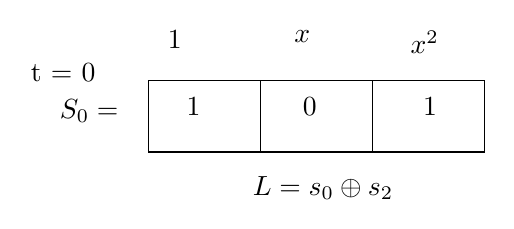
\begin{tikzpicture}[x=0.75pt,y=0.75pt,yscale=-1,xscale=1] 
        \draw   (255,893.6) -- (309,893.6) -- (309,928.2) -- (255,928.2) -- cycle ; 
        \draw   (309,893.6) -- (363,893.6) -- (363,928.2) -- (309,928.2) -- cycle ; 
        \draw   (363,893.6) -- (417,893.6) -- (417,928.2) -- (363,928.2) -- cycle ;
        
        \draw (328,900.6) node [anchor=north west][inner sep=0.75pt]   [align=left] {0};
        \draw (263,868.6) node [anchor=north west][inner sep=0.75pt]   [align=left] {1};
        \draw (324,868.6) node [anchor=north west][inner sep=0.75pt]   [align=left] {$x$};
        \draw (380,868.6) node [anchor=north west][inner sep=0.75pt]   [align=left] {$x^2$};
        \draw (197,884.6) node [anchor=north west][inner sep=0.75pt]   [align=left] {t = 0};
        \draw (211,901.6) node [anchor=north west][inner sep=0.75pt]   [align=left] {$S_0 = $};
        \draw (272,900.6) node [anchor=north west][inner sep=0.75pt]   [align=left] {1};
        \draw (386,900.6) node [anchor=north west][inner sep=0.75pt]   [align=left] {1};
        \draw (304,938.6) node [anchor=north west][inner sep=0.75pt]   [align=left] {$L = s_0 \oplus s_2$};
    \end{tikzpicture}
\end{center}
Therefore, the polynomial $g(x) = 1 + x^2$ and connecting polynomial $f(x) = x^3 + x + 1$.\\
    $1 \times g(x) = 1 + x^2$\\
    $x \times g(x) = x + x^3 = 1$\\
    $x^2 \times g(x) = x$\\
    $x^3 \times g(x) = x^2$\\
    $x^4 \times g(x) = x^3 = x + 1$\\
    $x^5 \times g(x) = x^2 + x$\\
    $x^6 \times g(x) = x^3 + x^2 = x^2 + x + 1$\\
    $x^7 \times g(x) = x^3 + x^2 + x = x + 1 + x^2 + x = 1 + x^2 = g(x)$\\
Since, after multiplication from $x^7$, g(x) is repeated again and $7 = 2^3 - 1$. Therefore, the given LFSR is fully periodic LFSR.\\
\textbf{Question} Suppose there is a non-zero state, and we are getting a period of $2^n - 1$. Is it guaranteed that period will be $2^n - 1$?\\
\textbf{Solution:} Yes, because all the states are generated in between these $2^n - 1$ states that are generated between the repetition of the given non-zero state. Hence, each state is repeated after $2^n - 1$ states. Hence, beginning with any state, the state will repeat after $2^n - 1$ states only. Hence, period will be $2^n - 1$.\\

\textbf{Example:}

\begin{center}
    \tikzset{every picture/.style={line width=0.75pt}}
    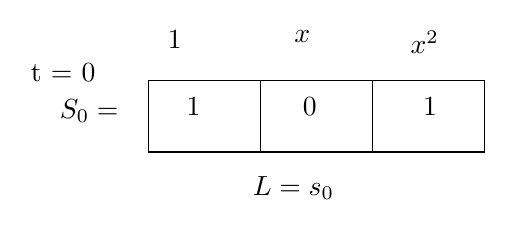
\begin{tikzpicture}[x=0.75pt,y=0.75pt,yscale=-1,xscale=1] 
        \draw   (255,893.6) -- (309,893.6) -- (309,928.2) -- (255,928.2) -- cycle ; 
        \draw   (309,893.6) -- (363,893.6) -- (363,928.2) -- (309,928.2) -- cycle ; 
        \draw   (363,893.6) -- (417,893.6) -- (417,928.2) -- (363,928.2) -- cycle ;
        
        \draw (328,900.6) node [anchor=north west][inner sep=0.75pt]   [align=left] {0};
        \draw (263,868.6) node [anchor=north west][inner sep=0.75pt]   [align=left] {1};
        \draw (324,868.6) node [anchor=north west][inner sep=0.75pt]   [align=left] {$x$};
        \draw (380,868.6) node [anchor=north west][inner sep=0.75pt]   [align=left] {$x^2$};
        \draw (197,884.6) node [anchor=north west][inner sep=0.75pt]   [align=left] {t = 0};
        \draw (211,901.6) node [anchor=north west][inner sep=0.75pt]   [align=left] {$S_0 = $};
        \draw (272,900.6) node [anchor=north west][inner sep=0.75pt]   [align=left] {1};
        \draw (386,900.6) node [anchor=north west][inner sep=0.75pt]   [align=left] {1};
        \draw (304,938.6) node [anchor=north west][inner sep=0.75pt]   [align=left] {$L = s_0$};
    \end{tikzpicture}
\end{center}
Therefore, the polynomial $g(x) = 1 + x^2$ and connecting polynomial $f(x) = x^3 + 1$.\\
    $1 \times g(x) = 1 + x^2$\\
    $x \times g(x) = x + x^3 = x + 1$\\
    $x^2 \times g(x) = x^2 + x$\\
    $x^3 \times g(x) = x^3 + x^2 = 1 + x^2 = g(x)$\\

Since, after multiplication from $x^3$, g(x) is repeated again and $7 \neq 2^3 - 1$. Therefore, the given LFSR is not fully periodic LFSR.\\

Let us now talk about the security of LFSR. Usually, we keep the secret key in the memory of LFSR, that is, in the register.

\begin{center}
    \tikzset{every picture/.style={line width=0.75pt}} 
    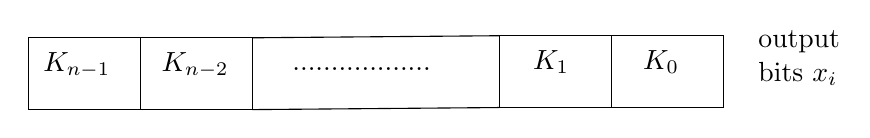
\begin{tikzpicture}[x=0.75pt,y=0.75pt,yscale=-1,xscale=1]
        \draw   (112,35) -- (166,35) -- (166,69.6) -- (112,69.6) -- cycle ; 
        \draw   (166,35) -- (220,35) -- (220,69.6) -- (166,69.6) -- cycle ;
        \draw   (339,34) -- (393,34) -- (393,68.6) -- (339,68.6) -- cycle ;
        \draw   (393,34) -- (447,34) -- (447,68.6) -- (393,68.6) -- cycle ;
        \draw    (220,69.6) -- (339,68.6) ;
        \draw    (220,35) -- (339,34) ;
        
        \draw (118,41) node [anchor=north west][inner sep=0.75pt]   [align=left] {$K_{n-1}$};
        \draw (175,41) node [anchor=north west][inner sep=0.75pt]   [align=left] {$K_{n-2}$};
        \draw (238,48) node [anchor=north west][inner sep=0.75pt]   [align=left] {..................};
        \draw (354,40) node [anchor=north west][inner sep=0.75pt]   [align=left] {$K_1$};
        \draw (407,40) node [anchor=north west][inner sep=0.75pt]   [align=left] {$K_0$};
        \draw (462.55,30.39) node [anchor=north west][inner sep=0.75pt]   [align=left] {output\\bits $x_i$};
    \end{tikzpicture}

    $K = K_0K_1.....K_{n-1}$
\end{center}

We will keep secret key or some other public parameter in the register and we will generate some bits.
\begin{center}
    output bits $x_i \rightarrow$ keystream bits $Z_i$\\
    $m_i \oplus Z_i = C_i \rightarrow$ ciphertext bits
\end{center}

Every time we will be clocking the LFSR, we will get one bit as output and will have feedback also. Now, if we consider Known Plaintext Attack Model, that is, we know certain plaintext bits and corresponding ciphertext bits and our aim is to find the secret key. Therefore, we know $m_i$ and $c_i$. Clearly,
\begin{center}
    $Z_i = m_i \oplus C_i$
\end{center}
Therefore, we know $Z_i$ corresponding to the know $m_i$ and $C_i$. Now, first output bit according to LFSR id $K_0$, the second output bit is $K_1$ and so on. That is, if we know the first n bits of the message and corresponding ciphertext, we can get entire secret key.\\
\newline
Even if we don't know the first n keystream bits, we can form a linear system of equations, because whatever bit we will get at leftmost position during clocking will be a linear function on the initial state only. For example, in the first clocking, 
\begin{center}
    $K_n = L(K_0, K_1,....., K_{n-1})$
\end{center}
and in the second clocking,
\begin{center}
    $K_{n+1} = L(K_1, K_2,....., K_n)$
\end{center}
but $K_n$ in again a linear combination of initial state only. Eventually, every bit coming to leftmost position is linear function on initial state only. Therfore, even if we know any key stream bits, that is any message bit and corresponding ciphertext bit, then,
\begin{center}
    $Z_i = m_i \oplus C_i$
\end{center}
and $Z_i$ will always be a linear function of $K_0, K_1,....., K_{n-1}$. If we know first n bits, $Z_i$ is a linear function with only one term ($K_0$ or $K_1$ or $K_{n-1}$). So, if we know $Z_i$ from known plaintext attack for any message bits. It is not required to know consecutive first n-bits. If we know any mesage bits and corresponding ciphertext bits, we can form a system of linear equations and solve that to get the secret key. Hence, simple LFSR does not provide good security.\\
\newline
Let us say you know one bit of message and corresponding ciphertext, that means you have only one linear equation. Let us say some $i^{th}$ bit (that is, not necessarily the first bit). Is is possible to reduce the search complexity of the secret key using that equation. The exhaustive search complexity of recovering the secret key is $2^n$ because this many keys are possible.\\
\newline
Let us say there is one $Z_i = 0$ and the linear equation formed is,
\begin{center}
    $Z_i = L(K_0, K_1,....., K_{n-1})$\\
    $0 = Z_i = K_2 \oplus K_6 \oplus K_{n-2}$\\
\end{center}
Using the linear equation, is it possible to reduce the complexity of searching the key? If we have correct guess for say $K_6$ and $K_{n-2}$, then $K_2$ is always determined. The search complexity, thus, is reduced to half.\\
Therefore, depending upon how many equations you are getting and the property of the system of equations, the search complexity will be reduced definitely. Therefore, knowing only 1 bit creates huge impact on the search complexity.\\
Say we have one system of linear equations with infinite solutions, so we will get all possible solutions here. So, if we have n variables but we have only few equations (say 5 or 6), still these equations will reduce the search complexity by a good margin. Therefore, using Known Plaintext Attack it is easy to break LFSR.\\

\subsubsection{LFSR with Non-Linear Filter Function}
Here, we will consider an l-bit boolean function $f$ which takes l-bits as input and produces one bit as output. We will take l-bits out of the n-bits of the state of LFSR as input to f and use the output of $f$ as $Z_i \in \{0, 1\}$. The function $f$ here is a non-linear function.
\begin{center}
    \tikzset{every picture/.style={line width=0.75pt}}        
    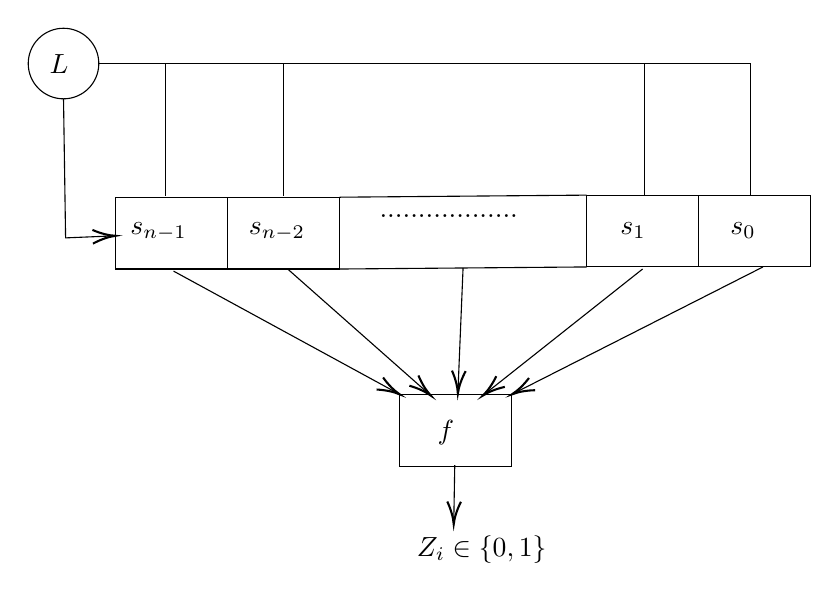
\begin{tikzpicture}[x=0.75pt,y=0.75pt,yscale=-1,xscale=1]
        \draw   (138,1067.4) -- (192,1067.4) -- (192,1102) -- (138,1102) -- cycle ;
        \draw   (192,1067.4) -- (246,1067.4) -- (246,1102) -- (192,1102) -- cycle ;
        \draw   (365,1066.4) -- (419,1066.4) -- (419,1101) -- (365,1101) -- cycle ;
        \draw    (246,1067.4) -- (365,1066.4) ;
        \draw   (419,1066.4) -- (473,1066.4) -- (473,1101) -- (419,1101) -- cycle ; 
        \draw    (246,1102) -- (365,1101) ;
        \draw    (166,1103) -- (273.24,1161.44) ;
        \draw [shift={(275,1162.4)}, rotate = 208.59] [color={rgb, 255:red, 0; green, 0; blue, 0 }  ][line width=0.75]    (10.93,-3.29) .. controls (6.95,-1.4) and (3.31,-0.3) .. (0,0) .. controls (3.31,0.3) and (6.95,1.4) .. (10.93,3.29)   ; 
        \draw    (130,1003) -- (444,1003) -- (444,1066.4) ;
        \draw   (96,1003) .. controls (96,993.61) and (103.61,986) .. (113,986) .. controls (122.39,986) and (130,993.61) .. (130,1003) .. controls (130,1012.39) and (122.39,1020) .. (113,1020) .. controls (103.61,1020) and (96,1012.39) .. (96,1003) -- cycle ;
        \draw    (113,1020) -- (114,1087) -- (136,1086.08) ;
        \draw [shift={(138,1086)}, rotate = 177.61] [color={rgb, 255:red, 0; green, 0; blue, 0 }  ][line width=0.75]    (10.93,-3.29) .. controls (6.95,-1.4) and (3.31,-0.3) .. (0,0) .. controls (3.31,0.3) and (6.95,1.4) .. (10.93,3.29)   ;
        \draw    (162,1003) -- (162,1067) ;
        \draw    (219,1003) -- (219,1067) ; 
        \draw    (393,1003) -- (393,1067) ; 
        \draw   (275,1162.4) -- (329,1162.4) -- (329,1197) -- (275,1197) -- cycle ; 
        \draw    (221,1102) -- (288.5,1161.68) ;
        \draw [shift={(290,1163)}, rotate = 221.48] [color={rgb, 255:red, 0; green, 0; blue, 0 }  ][line width=0.75]    (10.93,-3.29) .. controls (6.95,-1.4) and (3.31,-0.3) .. (0,0) .. controls (3.31,0.3) and (6.95,1.4) .. (10.93,3.29)   ;
        \draw    (392,1102) -- (316.57,1161.76) ;
        \draw [shift={(315,1163)}, rotate = 321.61] [color={rgb, 255:red, 0; green, 0; blue, 0 }  ][line width=0.75]    (10.93,-3.29) .. controls (6.95,-1.4) and (3.31,-0.3) .. (0,0) .. controls (3.31,0.3) and (6.95,1.4) .. (10.93,3.29)   ;
        \draw    (450,1101) -- (330.78,1161.49) ;
        \draw [shift={(329,1162.4)}, rotate = 333.1] [color={rgb, 255:red, 0; green, 0; blue, 0 }  ][line width=0.75]    (10.93,-3.29) .. controls (6.95,-1.4) and (3.31,-0.3) .. (0,0) .. controls (3.31,0.3) and (6.95,1.4) .. (10.93,3.29)   ;
        \draw    (305.5,1101.5) -- (303.08,1160) ;
        \draw [shift={(303,1162)}, rotate = 272.37] [color={rgb, 255:red, 0; green, 0; blue, 0 }  ][line width=0.75]    (10.93,-3.29) .. controls (6.95,-1.4) and (3.31,-0.3) .. (0,0) .. controls (3.31,0.3) and (6.95,1.4) .. (10.93,3.29)   ;
        \draw    (301.5,1196.5) -- (301.04,1223) ;
        \draw [shift={(301,1225)}, rotate = 271.01] [color={rgb, 255:red, 0; green, 0; blue, 0 }  ][line width=0.75]    (10.93,-3.29) .. controls (6.95,-1.4) and (3.31,-0.3) .. (0,0) .. controls (3.31,0.3) and (6.95,1.4) .. (10.93,3.29)   ;
        
        \draw (144,1078.4) node [anchor=north west][inner sep=0.75pt]   [align=left] {$s_{n-1}$};
        \draw (201,1078.4) node [anchor=north west][inner sep=0.75pt]   [align=left] {$s_{n-2}$};
        \draw (264,1074.4) node [anchor=north west][inner sep=0.75pt]   [align=left] {..................};
        \draw (380,1078.4) node [anchor=north west][inner sep=0.75pt]   [align=left] {$s_1$};
        \draw (433,1078.4) node [anchor=north west][inner sep=0.75pt]   [align=left] {$s_0$};
        \draw (105,997.4) node [anchor=north west][inner sep=0.75pt]   [align=left] {$L$};
        \draw (282,1229.4) node [anchor=north west][inner sep=0.75pt]   [align=left] {$Z_i \in \{0,1\}$};
        \draw (292,1173.4) node [anchor=north west][inner sep=0.75pt]   [align=left] {$f$};
    \end{tikzpicture}\\
    \vspace{2mm}
    $f: \{0, 1\}^l \rightarrow \{0, 1\}$\\
    \vspace{1mm}
    $n \geq l$\\
    \vspace{1mm}
    $C_i = m_i \oplus Z_i$
\end{center}

The state update function of LFSR will be same - there will be linear feedback function (L) and shifting as earlier. Therefore, if we select $l$ fixed position from the $n$ positions in the register, at each clocking the value at these position will update. If the function $f$ is good enough, the output will still be random looking. In fact, this will also have full period if $f$ is a good function and the connection polynomial corresponding to $L$ is primitive.\\
\newline
The advantage here is that even if we know $m_i$ and corresponding $c_i$ from Known Plaintext Attack model, and consequently we know $Z_i$. The $Z_i$ is now a non-linear function of state bits of LFSR. Solving a non-linear system of equation might be computationally difficult.\\
\newline
The state update function of LFSR is, say $\alpha$. Therefore, 
\begin{center}
    $S_{t+1} = \alpha(S_t)$\\
    $Z_{t+1} = f(S_{t+1})$
\end{center}
Let us look at the LFSR state at clocking time t.
\begin{center}
    $S_t = (s_{n-1}^t, s_{n-2}^t,....., s_0^t)$
\end{center}
The state of LFSR at clocking time (t+1) will be, 
\begin{center}
    $S_{t+1} = (s_{n-1}^{t+1}, s_{n-2}^{t+1},....., s_0^{t+1})$
\end{center}
Suppose the shifting to be right shift, therefore, 
\begin{center}
    $s_0^{t+1} = s_1^t, s_1^{t+1} = s_2^t,....,s_{n-2}^{t+1} = s_{n-1}^t, s_{n-1}^{t+1} = L(s_{n-1}^t, s_{n-2}^t,....., s_0^t)$
\end{center}
The state update can be represented as a matrix multiplication in the following way,
\begin{center}
    $ S^{t+1} = 
    \begin{bmatrix}
        s_0^{t+1}\\
        s_1^{t+1}\\
        \vdots\\
        S_{n-1}^{t+1}\\
    \end{bmatrix}
    =
    \begin{bmatrix}
        0 & 1 & 0 & 0 & \hdots & 0\\
        0 & 0 & 1 & 0 & \hdots & 0\\
        0 & 0 & 0 & 1 & \hdots & 0\\
        \vdots & \vdots & \vdots & \vdots & \ddots & \vdots\\
        0 & 0 & 0 & 0 & \hdots & 1\\
        c_n & c_{n-1} & c_{n-2} & c_{n-3} & \hdots & c_1\\
    \end{bmatrix}
    \begin{bmatrix}
        s_0^{t}\\
        s_1^{t}\\
        \vdots\\
        S_{n-1}^{t}\\
    \end{bmatrix}
    $\\
    \vspace{2mm}
    $L = c_n\cdot s_0 \oplus c_{n-1} \cdot s_1 \oplus \hdots \oplus c_1\cdot s_{n-1}$
\end{center}

\subsubsection{LFSR with Combiner Function}
We have a similar function $f$ as we discussed above. However, here we have $l$ number of LFSR's. The output of these $l$ LFSR's, that is, l-bits becomes the input for the combiner function $f$ whose output is treated as $Z_i$. The function $f$ is non-linear.

\begin{center}
    \tikzset{every picture/.style={line width=0.75pt}}
    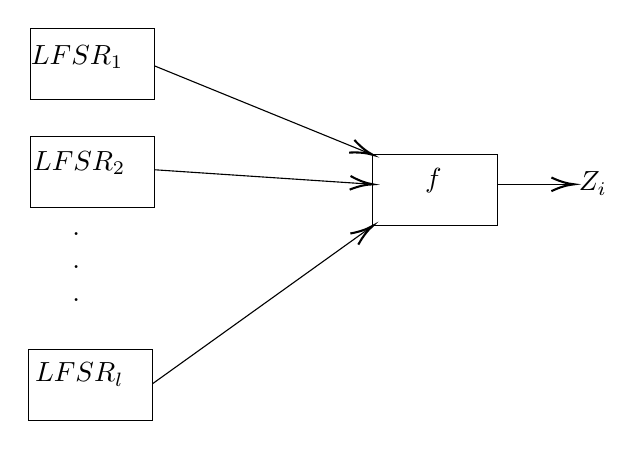
\begin{tikzpicture}[x=0.75pt,y=0.75pt,yscale=-1,xscale=1]
        \draw   (121,47) -- (181,47) -- (181,81.2) -- (121,81.2) -- cycle ;
        \draw   (120,202) -- (180,202) -- (180,236.2) -- (120,236.2) -- cycle ;
        \draw   (121,99) -- (181,99) -- (181,133.2) -- (121,133.2) -- cycle ;
        \draw   (286,108) -- (346,108) -- (346,142.2) -- (286,142.2) -- cycle ;
        \draw    (181,65.2) -- (284.15,107.25) ;
        \draw [shift={(286,108)}, rotate = 202.18] [color={rgb, 255:red, 0; green, 0; blue, 0 }  ][line width=0.75]    (10.93,-3.29) .. controls (6.95,-1.4) and (3.31,-0.3) .. (0,0) .. controls (3.31,0.3) and (6.95,1.4) .. (10.93,3.29)   ;
        \draw    (181,115.2) -- (284,122.07) ;
        \draw [shift={(286,122.2)}, rotate = 183.81] [color={rgb, 255:red, 0; green, 0; blue, 0 }  ][line width=0.75]    (10.93,-3.29) .. controls (6.95,-1.4) and (3.31,-0.3) .. (0,0) .. controls (3.31,0.3) and (6.95,1.4) .. (10.93,3.29)   ;
        \draw    (180,218.2) -- (284.37,143.37) ;
        \draw [shift={(286,142.2)}, rotate = 144.36] [color={rgb, 255:red, 0; green, 0; blue, 0 }  ][line width=0.75]    (10.93,-3.29) .. controls (6.95,-1.4) and (3.31,-0.3) .. (0,0) .. controls (3.31,0.3) and (6.95,1.4) .. (10.93,3.29)   ;
        \draw    (346,122.2) -- (381,122.2) ;
        \draw [shift={(383,122.2)}, rotate = 180] [color={rgb, 255:red, 0; green, 0; blue, 0 }  ][line width=0.75]    (10.93,-3.29) .. controls (6.95,-1.4) and (3.31,-0.3) .. (0,0) .. controls (3.31,0.3) and (6.95,1.4) .. (10.93,3.29)   ;
        
        \draw (120,54) node [anchor=north west][inner sep=0.75pt]   [align=left] {$LFSR_1$};
        \draw (121,105) node [anchor=north west][inner sep=0.75pt]   [align=left] {$LFSR_2$};
        \draw (122,207) node [anchor=north west][inner sep=0.75pt]   [align=left] {$LFSR_l$};
        \draw (310,113) node [anchor=north west][inner sep=0.75pt]   [align=left] {$f$};
        \draw (140,144) node [anchor=north west][inner sep=0.75pt]   [align=left] {.\\.\\.};
        \draw (384,115) node [anchor=north west][inner sep=0.75pt]   [align=left] {$Z_i$};
    \end{tikzpicture}\\
    $C_i = m_i \oplus Z_i$
\end{center}    

\textbf{Example:} Consider the following 3-LFSR with non-liner filter function $f$.
\begin{center}
    \tikzset{every picture/.style={line width=0.75pt}}       
    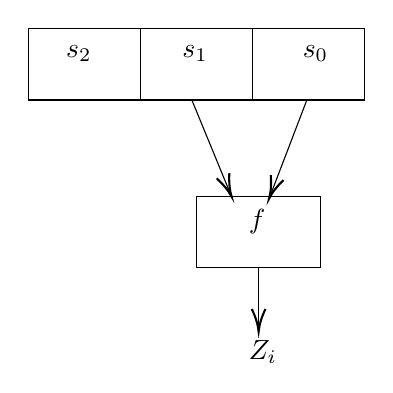
\begin{tikzpicture}[x=0.75pt,y=0.75pt,yscale=-1,xscale=1]
        \draw   (444,57) -- (498,57) -- (498,91.6) -- (444,91.6) -- cycle ;
        \draw   (498,57) -- (552,57) -- (552,91.6) -- (498,91.6) -- cycle ;
        \draw   (552,57) -- (606,57) -- (606,91.6) -- (552,91.6) -- cycle ;
        \draw   (525,138) -- (585,138) -- (585,172.2) -- (525,172.2) -- cycle ;
        \draw    (523,92) -- (541.24,136.35) ;
        \draw [shift={(542,138.2)}, rotate = 247.64] [color={rgb, 255:red, 0; green, 0; blue, 0 }  ][line width=0.75]    (10.93,-3.29) .. controls (6.95,-1.4) and (3.31,-0.3) .. (0,0) .. controls (3.31,0.3) and (6.95,1.4) .. (10.93,3.29)   ;
        \draw    (578,92.2) -- (560.72,137.33) ;
        \draw [shift={(560,139.2)}, rotate = 290.96] [color={rgb, 255:red, 0; green, 0; blue, 0 }  ][line width=0.75]    (10.93,-3.29) .. controls (6.95,-1.4) and (3.31,-0.3) .. (0,0) .. controls (3.31,0.3) and (6.95,1.4) .. (10.93,3.29)   ;
        \draw    (555,172) -- (555,201.2) ;
        \draw [shift={(555,203.2)}, rotate = 270] [color={rgb, 255:red, 0; green, 0; blue, 0 }  ][line width=0.75]    (10.93,-3.29) .. controls (6.95,-1.4) and (3.31,-0.3) .. (0,0) .. controls (3.31,0.3) and (6.95,1.4) .. (10.93,3.29)   ;
        
        \draw (517,64) node [anchor=north west][inner sep=0.75pt]   [align=left] {$s_1$};
        \draw (461,64) node [anchor=north west][inner sep=0.75pt]   [align=left] {$s_2$};
        \draw (575,64) node [anchor=north west][inner sep=0.75pt]   [align=left] {$s_0$};
        \draw (549,143) node [anchor=north west][inner sep=0.75pt]   [align=left] {$f$};
        \draw (549,206) node [anchor=north west][inner sep=0.75pt]   [align=left] {$Z_i$};
    \end{tikzpicture}\\
    $f: \{0,1\}^2 \rightarrow \{0,1\}$\\
    $f(x_0, x_1) = x_0 \cdot x_1$
\end{center}
Here, if we draw the truth table of $f$, it will look like,

\begin{table}[h]
\centering
  \begin{tabular}{c|c||c}
        \textbf{$x_0$} & \textbf{$x_1$} & \textbf{$f$} \\
        \hline
        0 & 0 & 0 \\
        0 & 1 & 0 \\
        1 & 0 & 0 \\
        1 & 1 & 1 \\
  \end{tabular}
\end{table}
We can see that $Pr[Z = 0] = \frac{3}{4}$. Here, $f$ is not a good function because $Pr[Z = 0] > Pr[Z = 1]$, that is, it is highly biased. We need to design $f$ such that the output is unpredictable. Here, we can predict that output will be zero with a higher probability. If we have a stream cipher with this model and we are able to find out the $f$ function. We can eventually break the stream cipher. Therefore, $f$ must be selected carefully.

\subsection{Non-Linear Feedback Shift Register}
After a few years, it was observed that LFSRs are good ciphers which are still secure but most of the ciphers can be broken using various adverse cryptanalysis techniques.\\
\newline
To prevent all this, there is a concept of stream ciphers known as Non-Linear Feedback Shift Register (NFSR's). From the name, it can be anticipated that the feedback function will be non-linear in NFSR. In fact, in modern scenarios, all stream ciphers are based on NFSR.\\
\newline
In NFSR, the mechanism is similar to LFSR, but the feedback is non-linear. \\
\textbf{Note: } The problem in NFSR is that if we consider a Non-Linear Feedback Function, there is no methodical proof which can determine the period of NFSR. For LFSR, if the connection polynomial is primitive, then the LFSR is fully periodic. In case of NFSR, we don't have any such proof or method.

\subsubsection{Grain}
Grain is a standard stream cipher which with an 80-bit key and a 64-bit IV. In block ciphers, there is only one standard algorithm, that is, the AES. There are other good block cipher algorithms that are as secure as AES, but they are not efficient. However, in stream ciphers, multiple ciphers are standardized. In fact, in most mobile and hardware devices, you will find some non-standardized stream cipher. In most 4G mobile phones, stream ciphers are based on ZUC stream cipher which is not a standardized stream cipher.\\
\newline
The design of Grain is based on NFSR with LFSR and a non-linear combiner function. Although the design is a little complicated, but its implementation is extremely efficient. Let us look into the design of Grain.

\begin{center}
    \tikzset{every picture/.style={line width=0.75pt}}         
    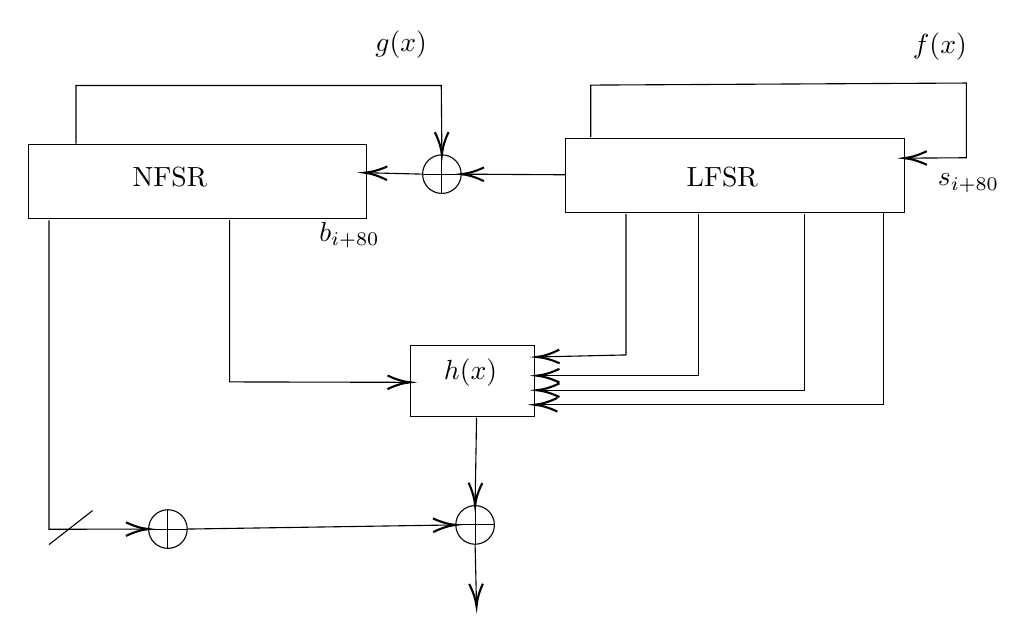
\begin{tikzpicture}[x=0.75pt,y=0.75pt,yscale=-1,xscale=1]
        \draw   (102,432.2) -- (265,432.2) -- (265,467.8) -- (102,467.8) -- cycle ;
        \draw   (361,429.2) -- (524,429.2) -- (524,464.8) -- (361,464.8) -- cycle ;
        \draw   (286,529) -- (346,529) -- (346,563.2) -- (286,563.2) -- cycle ;
        \draw   (292,446.5) .. controls (292,441.36) and (296.16,437.2) .. (301.3,437.2) .. controls (306.44,437.2) and (310.6,441.36) .. (310.6,446.5) .. controls (310.6,451.64) and (306.44,455.8) .. (301.3,455.8) .. controls (296.16,455.8) and (292,451.64) .. (292,446.5) -- cycle ; \draw   (292,446.5) -- (310.6,446.5) ; \draw   (301.3,437.2) -- (301.3,455.8) ;
        \draw   (308,615.5) .. controls (308,610.36) and (312.16,606.2) .. (317.3,606.2) .. controls (322.44,606.2) and (326.6,610.36) .. (326.6,615.5) .. controls (326.6,620.64) and (322.44,624.8) .. (317.3,624.8) .. controls (312.16,624.8) and (308,620.64) .. (308,615.5) -- cycle ; \draw   (308,615.5) -- (326.6,615.5) ; \draw   (317.3,606.2) -- (317.3,624.8) ;
        \draw   (160,617.5) .. controls (160,612.36) and (164.16,608.2) .. (169.3,608.2) .. controls (174.44,608.2) and (178.6,612.36) .. (178.6,617.5) .. controls (178.6,622.64) and (174.44,626.8) .. (169.3,626.8) .. controls (164.16,626.8) and (160,622.64) .. (160,617.5) -- cycle ; \draw   (160,617.5) -- (178.6,617.5) ; \draw   (169.3,608.2) -- (169.3,626.8) ;
        \draw    (178.6,617.5) -- (306,615.53) ;
        \draw [shift={(308,615.5)}, rotate = 179.11] [color={rgb, 255:red, 0; green, 0; blue, 0 }  ][line width=0.75]    (10.93,-3.29) .. controls (6.95,-1.4) and (3.31,-0.3) .. (0,0) .. controls (3.31,0.3) and (6.95,1.4) .. (10.93,3.29)   ;
        \draw    (112,468.8) -- (112,617.6) -- (158,617.5) ;
        \draw [shift={(160,617.5)}, rotate = 179.88] [color={rgb, 255:red, 0; green, 0; blue, 0 }  ][line width=0.75]    (10.93,-3.29) .. controls (6.95,-1.4) and (3.31,-0.3) .. (0,0) .. controls (3.31,0.3) and (6.95,1.4) .. (10.93,3.29)   ;
        \draw    (112,625) -- (133,608.6) ;
        \draw    (390,465.6) -- (390,533.6) -- (349,534.55) ;
        \draw [shift={(347,534.6)}, rotate = 358.67] [color={rgb, 255:red, 0; green, 0; blue, 0 }  ][line width=0.75]    (10.93,-3.29) .. controls (6.95,-1.4) and (3.31,-0.3) .. (0,0) .. controls (3.31,0.3) and (6.95,1.4) .. (10.93,3.29)   ;
        \draw    (425,465.6) -- (425,543.6) -- (349,543.6) ;
        \draw [shift={(347,543.6)}, rotate = 360] [color={rgb, 255:red, 0; green, 0; blue, 0 }  ][line width=0.75]    (10.93,-3.29) .. controls (6.95,-1.4) and (3.31,-0.3) .. (0,0) .. controls (3.31,0.3) and (6.95,1.4) .. (10.93,3.29)   ;
        \draw    (476,465.6) -- (476,550.6) -- (349,550.6) ;
        \draw [shift={(347,550.6)}, rotate = 360] [color={rgb, 255:red, 0; green, 0; blue, 0 }  ][line width=0.75]    (10.93,-3.29) .. controls (6.95,-1.4) and (3.31,-0.3) .. (0,0) .. controls (3.31,0.3) and (6.95,1.4) .. (10.93,3.29)   ;
        \draw    (514,464.6) -- (514,557.6) -- (348,557.6) ;
        \draw [shift={(346,557.6)}, rotate = 360] [color={rgb, 255:red, 0; green, 0; blue, 0 }  ][line width=0.75]    (10.93,-3.29) .. controls (6.95,-1.4) and (3.31,-0.3) .. (0,0) .. controls (3.31,0.3) and (6.95,1.4) .. (10.93,3.29)   ;
        \draw    (373,428.6) -- (373,403.6) -- (554,402.6) -- (554,438.6) -- (526,438.79) ;
        \draw [shift={(524,438.8)}, rotate = 359.62] [color={rgb, 255:red, 0; green, 0; blue, 0 }  ][line width=0.75]    (10.93,-3.29) .. controls (6.95,-1.4) and (3.31,-0.3) .. (0,0) .. controls (3.31,0.3) and (6.95,1.4) .. (10.93,3.29)   ;
        \draw    (125,431.8) -- (125,403.8) -- (301,403.8) -- (301.28,435.2) ;
        \draw [shift={(301.3,437.2)}, rotate = 269.49] [color={rgb, 255:red, 0; green, 0; blue, 0 }  ][line width=0.75]    (10.93,-3.29) .. controls (6.95,-1.4) and (3.31,-0.3) .. (0,0) .. controls (3.31,0.3) and (6.95,1.4) .. (10.93,3.29)   ;
        \draw    (292,446.5) -- (266,445.85) ;
        \draw [shift={(264,445.8)}, rotate = 1.43] [color={rgb, 255:red, 0; green, 0; blue, 0 }  ][line width=0.75]    (10.93,-3.29) .. controls (6.95,-1.4) and (3.31,-0.3) .. (0,0) .. controls (3.31,0.3) and (6.95,1.4) .. (10.93,3.29)   ;
        \draw    (361,446.8) -- (312.6,446.51) ;
        \draw [shift={(310.6,446.5)}, rotate = 0.34] [color={rgb, 255:red, 0; green, 0; blue, 0 }  ][line width=0.75]    (10.93,-3.29) .. controls (6.95,-1.4) and (3.31,-0.3) .. (0,0) .. controls (3.31,0.3) and (6.95,1.4) .. (10.93,3.29)   ;
        \draw    (199,468.6) -- (199,546.6) -- (284,546.8) ;
        \draw [shift={(286,546.8)}, rotate = 180.13] [color={rgb, 255:red, 0; green, 0; blue, 0 }  ][line width=0.75]    (10.93,-3.29) .. controls (6.95,-1.4) and (3.31,-0.3) .. (0,0) .. controls (3.31,0.3) and (6.95,1.4) .. (10.93,3.29)   ;
        \draw    (318,563.8) -- (317.33,604.2) ;
        \draw [shift={(317.3,606.2)}, rotate = 270.95] [color={rgb, 255:red, 0; green, 0; blue, 0 }  ][line width=0.75]    (10.93,-3.29) .. controls (6.95,-1.4) and (3.31,-0.3) .. (0,0) .. controls (3.31,0.3) and (6.95,1.4) .. (10.93,3.29)   ;
        \draw    (317.3,624.8) -- (317.95,652.8) ;
        \draw [shift={(318,654.8)}, rotate = 268.66] [color={rgb, 255:red, 0; green, 0; blue, 0 }  ][line width=0.75]    (10.93,-3.29) .. controls (6.95,-1.4) and (3.31,-0.3) .. (0,0) .. controls (3.31,0.3) and (6.95,1.4) .. (10.93,3.29)   ;
        
        \draw (151,442.2) node [anchor=north west][inner sep=0.75pt]   [align=left] {NFSR};
        \draw (418,442.2) node [anchor=north west][inner sep=0.75pt]   [align=left] {LFSR};
        \draw (301,534.2) node [anchor=north west][inner sep=0.75pt]   [align=left] {$h(x)$};
        \draw (268,376.2) node [anchor=north west][inner sep=0.75pt]   [align=left] {$g(x)$};
        \draw (527,377.2) node [anchor=north west][inner sep=0.75pt]   [align=left] {$f(x)$};
        \draw (539,445.2) node [anchor=north west][inner sep=0.75pt]   [align=left] {$s_{i+80}$};
        \draw (241,468.2) node [anchor=north west][inner sep=0.75pt]   [align=left] {$b_{i+80}$};
    \end{tikzpicture}
\end{center}

The NFSR and LFSR are each 80-bit. The connection polynomial corresponding to LFSR is primitive and hence LFSR is fully periodic. The function $g(x)$ is non-linear feedback function  of NFSR and the function $f(x)$ is linear feedback function of LFSR. If we say that cipher is clocked, it means that both NFSR and LFSR are clocked. Both LFSR and NFSR are shifted towards left.\\
\newline
In every clocking, it takes 1 bit from the NFSR and 4 bits from LFSR and pass it to $h(x)$. The position of these bits are fixed. $h(x)$ is also a non-linear filter function. It will produce 1-bit output. This bit will be xored by the 7-bits from the NFSR (the line with a little slash). The 7-bits from NFSR are taken from fixed position and are xored and then the output is zored with the output of $h(x)$.\\
\newline



The content of the LFSR is denoted by $s_i, s_{i+1}, . . . , s_{i+79}$ and the content of the NFSR is denoted by $b_i, b_{i+1}, . . . , b_{i+79}$.
The feedback (connection) polynomial of the LFSR, $f(x)$ is a primitive polynomial of degree
80. It is defined as:
\begin{center}
    $f(x) = 1 + x_{18} + x_{29} + x_{42} + x_{57} + x_{67} + x_{80}$
\end{center}
Therefore, the state update function of LFSR is:
\begin{center}
    $s_{i+80} = s_{i+62} + s_{i+51} + s_{i+38} + s_{i+23} + s_{i+13} + s_i$
\end{center}

The feedback polynomial of the NFSR, $g(x)$, is defined as:
\begin{center}
    $g(x) = 1 \oplus x^{18} \oplus x^{20} \oplus x^{28} \oplus x^{35} \oplus x^{43} \oplus x^{47} \oplus x^{52} \oplus x^{59} \oplus x^{66} \oplus x^{71} \oplus x^{80} \oplus x^{17}x^{20} \oplus x^{43}x^{47} \oplus x^{65}x^{71} \oplus x^{20}x^{28}x^{35} \oplus x^{47}x^{52}x^{59} \oplus x^{17}x^{35}x^{52}x^{71} \oplus x^{20}x^{28}x^{43}x^{47} \oplus x^{17}x^{20}x^{59}x^{65} \oplus x^{17}x^{20}x^{28}x^{35}x^{43} \oplus x^{47}x^{52}x^{59}x^{65}x^{71} \oplus x^{28}x^{35}x^{43}x^{47}x^{52}x^{59}$
\end{center}
The state update function of NFSR is:
\begin{center}
   $b_{i+80} = s_i \oplus b_{i+62} \oplus b_{i+60} \oplus b_{i+52} \oplus b_{i+45} \oplus b_{i+37} \oplus b_{i+33} \oplus b_{i+28} \oplus b_{i+21} \oplus b_{i+14} \oplus b_{i+9} \oplus b_i \oplus b_{i+63}b_{i+60} \oplus b_{i+37}b_{i+33} \oplus b_{i+15}b_{i+9} \oplus b_{i+60}b_{i+52}b_{i+45} \oplus b_{i+33}b_{i+28}b_{i+21} \oplus b_{i+63}b_{i+45}b_{i+28}b_{i+9} \oplus b_{i+60}b_{i+52}b_{i+37}b_{i+33} \oplus b_{i+63}b_{i+60}b_{i+21}b_{i+15} \oplus b_{i+63}b_{i+60}b_{i+52}b_{i+45}b_{i+37} \oplus b_{i+33}b_{i+28}b_{i+21}b_{i+15}b_{i+9} \oplus b_{i+52}b_{i+45}b_{i+37}b_{i+33}b_{i+28}b_{i+21}$ 
\end{center}
The feedback bit in NFSR is not just the non-linear feedback function of NFSR. The output of the non-linear feedback function is xored with the output bit (not the feedback bit) of LFSR, that is, $s_i$.\\
\newline
The contents of the two shift registers represent the state of the cipher. From
this state, 5 variables are taken as input to a boolean function, $h(x)$. The function $h(x)$ is a degree 3 function defined as:
\begin{center}
    $h(x) = x_1 \oplus x_4 \oplus x_0x_3 \oplus x_2x_3 \oplus x_3x_4 \oplus x_0x_1x_2 \oplus x_0x_2x_3 \oplus x_0x_2x_4 \oplus x_1x_2x_4 \oplus x_2x_3x_4$
\end{center}
where the variables $x_0, x_1, x_2, x_3$ and $x_4$ correspond to the tap positions $s_{i+3},
s_{i+25}, s_{i+46}, s_{i+64}$ and $b_{i+63}$ respectively. The output function is taken as:
\begin{center}
    $Z_i =  \sum_{k \in A} b_{i+k} \oplus h(s_{i+3},s_{i+25}, s_{i+46}, s_{i+64}, b_{i+63})$
\end{center}
where $A = \{1, 2, 4, 10, 31, 43, 56\}$.\\
\newline
The NFSR stream cipher is a good cipher but we don't have any proof for finding its period. But because of LFSR, we can claim that its period will be at least $2^{80} - 1$.\\
\newline
In most of the standardized stream ciphers, there are two phases:
\begin{itemize}
    \item \textbf{Key IV Initialization Phase:} In Key IV (or Key) Initialization Phase the cipher initializes its state. In this phase, the cipher is initialized automatically. That is, certain bits will be put in the state and it will update the state in a peculiar way and generate a random looking state.
    \item \textbf{Keystream Generation Phase:} In Keystream Generation Phase, the cipher produces output bits (keystream bits, $Z_i$) which are used for encryption. 
\end{itemize}

\subsubsubsection{Key IV Initialization Phase of Grain}
Before any keystream is generated the cipher must be initialized with the key and the IV. Let the key be K and Initialization Vector be IV. The bits of K and IV can be represented as:
\begin{center}
    $K_i, 0 \leq i \leq 79$\\
    $IV_i, 0 \leq i \leq 63$
\end{center}
The initialization of the key is done as follows. First, we load the NFSR with the key bits, $b_i = k_i, 0 \leq i \leq 79$, then load the first 64 bits of the LFSR with the IV, $s_i = IV_i, 0 \leq i \leq 63$. The remaining bits of the LFSR are filled with ones, $s_i = 1, 64 \leq i \leq 79$. We know that if LFSR is in zero state, then it remains in zero state. Hence, to avoid LFSR being in zero state, the remaining 16 bits are filled with 1. Now, since we know the LFSR is fully periodic, hence it will never be in zero state.\\
\newline
At each clocking, we know the cipher will produce a single bit output, which in the Keystream Generation Phase is $Z_i$. However, in Key IV Initialization phase, this output is fed back and xored with the input, both to the LFSR and NFSR.

\begin{center}
    \tikzset{every picture/.style={line width=0.75pt}}
    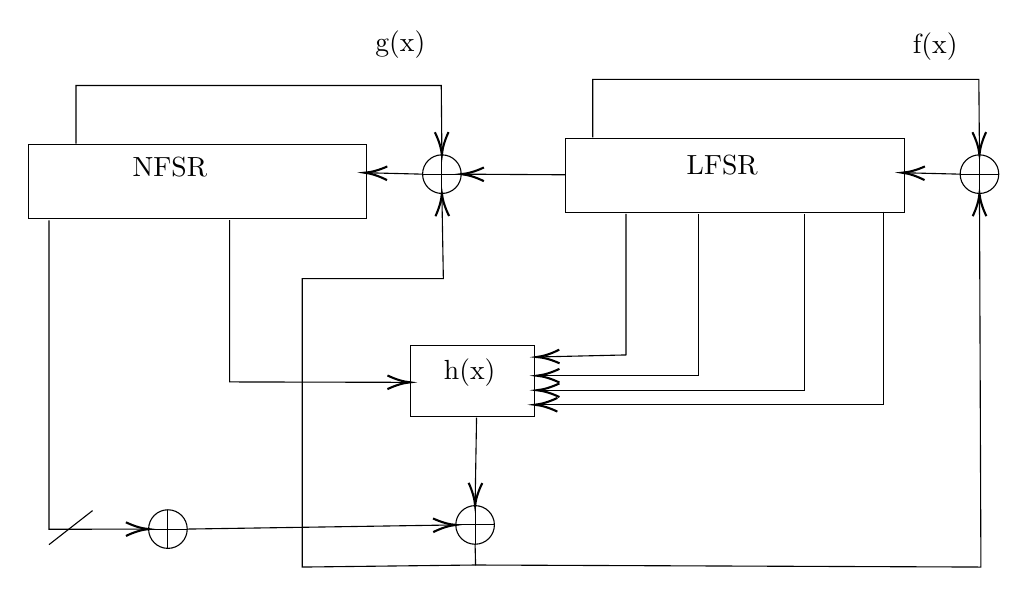
\begin{tikzpicture}[x=0.75pt,y=0.75pt,yscale=-1,xscale=1]
        \draw (86,800) -- (249,800) -- (249,835.6) -- (86,835.6) -- cycle ;
        \draw (345,797) -- (508,797) -- (508,832.6) -- (345,832.6) -- cycle ;
        \draw (270,896.8) -- (330,896.8) -- (330,931) -- (270,931) -- cycle ;
        \draw (276,814.3) .. controls (276,809.16) and (280.16,805) .. (285.3,805) .. controls (290.44,805) and (294.6,809.16) .. (294.6,814.3) .. controls (294.6,819.44) and (290.44,823.6) .. (285.3,823.6) .. controls (280.16,823.6) and (276,819.44) .. (276,814.3) -- cycle ;
        \draw (276,814.3) -- (294.6,814.3) ;
        \draw (285.3,805) -- (285.3,823.6) ;
        \draw (292,983.3) .. controls (292,978.16) and (296.16,974) .. (301.3,974) .. controls (306.44,974) and (310.6,978.16) .. (310.6,983.3) .. controls (310.6,988.44) and (306.44,992.6) .. (301.3,992.6) .. controls (296.16,992.6) and (292,988.44) .. (292,983.3) -- cycle ;
        \draw (292,983.3) -- (310.6,983.3) ;
        \draw (301.3,974) -- (301.3,992.6) ;
        \draw (144,985.3) .. controls (144,980.16) and (148.16,976) .. (153.3,976) .. controls (158.44,976) and (162.6,980.16) .. (162.6,985.3) .. controls (162.6,990.44) and (158.44,994.6) .. (153.3,994.6) .. controls (148.16,994.6) and (144,990.44) .. (144,985.3) -- cycle ;
        \draw (144,985.3) -- (162.6,985.3) ;
        \draw (153.3,976) -- (153.3,994.6) ;
        \draw (162.6,985.3) -- (290,983.33) ;
        \draw [shift={(292,983.3)}, rotate = 179.11] [color={rgb, 255:red, 0; green, 0; blue, 0 }  ][line width=0.75]    (10.93,-3.29) .. controls (6.95,-1.4) and (3.31,-0.3) .. (0,0) .. controls (3.31,0.3) and (6.95,1.4) .. (10.93,3.29)   ;
        \draw    (96,836.6) -- (96,985.4) -- (142,985.3) ;
        \draw [shift={(144,985.3)}, rotate = 179.88] [color={rgb, 255:red, 0; green, 0; blue, 0 } ][line width=0.75] (10.93,-3.29) .. controls (6.95,-1.4) and (3.31,-0.3) .. (0,0) .. controls (3.31,0.3) and (6.95,1.4) .. (10.93,3.29) ;
        \draw (96,992.8) -- (117,976.4) ;
        \draw (374,833.4) -- (374,901.4) -- (333,902.35) ;
        \draw [shift={(331,902.4)}, rotate = 358.67] [color={rgb, 255:red, 0; green, 0; blue, 0 } ][line width=0.75] (10.93,-3.29) .. controls (6.95,-1.4) and (3.31,-0.3) .. (0,0) .. controls (3.31,0.3) and (6.95,1.4) .. (10.93,3.29) ;
        \draw (409,833.4) -- (409,911.4) -- (333,911.4) ;
        \draw [shift={(331,911.4)}, rotate = 360] [color={rgb, 255:red, 0; green, 0; blue, 0 } ][line width=0.75] (10.93,-3.29) .. controls (6.95,-1.4) and (3.31,-0.3) .. (0,0) .. controls (3.31,0.3) and (6.95,1.4) .. (10.93,3.29) ;
        \draw (460,833.4) -- (460,918.4) -- (333,918.4) ;
        \draw [shift={(331,918.4)}, rotate = 360] [color={rgb, 255:red, 0; green, 0; blue, 0 } ][line width=0.75] (10.93,-3.29) .. controls (6.95,-1.4) and (3.31,-0.3) .. (0,0) .. controls (3.31,0.3) and (6.95,1.4) .. (10.93,3.29);
        \draw (498,832.4) -- (498,925.4) -- (332,925.4) ;
        \draw [shift={(330,925.4)}, rotate = 360] [color={rgb, 255:red, 0; green, 0; blue, 0 } ][line width=0.75] (10.93,-3.29) .. controls (6.95,-1.4) and (3.31,-0.3) .. (0,0) .. controls (3.31,0.3) and (6.95,1.4) .. (10.93,3.29);
        \draw (109,799.6) -- (109,771.6) -- (285,771.6) -- (285.28,803) ;
        \draw [shift={(285.3,805)}, rotate = 269.49] [color={rgb, 255:red, 0; green, 0; blue, 0 } ][line width=0.75] (10.93,-3.29) .. controls (6.95,-1.4) and (3.31,-0.3) .. (0,0) .. controls (3.31,0.3) and (6.95,1.4) .. (10.93,3.29);
        \draw (276,814.3) -- (250,813.65) ;
        \draw [shift={(248,813.6)}, rotate = 1.43] [color={rgb, 255:red, 0; green, 0; blue, 0 } ][line width=0.75] (10.93,-3.29) .. controls (6.95,-1.4) and (3.31,-0.3) .. (0,0) .. controls (3.31,0.3) and (6.95,1.4) .. (10.93,3.29);
        \draw (345,814.6) -- (296.6,814.31) ;
        \draw [shift={(294.6,814.3)}, rotate = 0.34] [color={rgb, 255:red, 0; green, 0; blue, 0 } ][line width=0.75] (10.93,-3.29) .. controls (6.95,-1.4) and (3.31,-0.3) .. (0,0) .. controls (3.31,0.3) and (6.95,1.4) .. (10.93,3.29) ;
        \draw (183,836.4) -- (183,914.4) -- (268,914.6) ;
        \draw [shift={(270,914.6)}, rotate = 180.13] [color={rgb, 255:red, 0; green, 0; blue, 0 } ][line width=0.75] (10.93,-3.29) .. controls (6.95,-1.4) and (3.31,-0.3) .. (0,0) .. controls (3.31,0.3) and (6.95,1.4) .. (10.93,3.29) ;
        \draw (302,931.6) -- (301.33,972) ;
        \draw [shift={(301.3,974)}, rotate = 270.95] [color={rgb, 255:red, 0; green, 0; blue, 0 } ][line width=0.75] (10.93,-3.29) .. controls (6.95,-1.4) and (3.31,-0.3) .. (0,0) .. controls (3.31,0.3) and (6.95,1.4) .. (10.93,3.29) ;
        \draw (301.3,992.6) -- (301.53,1002.61) -- (545,1003.6) -- (544.31,825.6) ;
        \draw [shift={(544.3,823.6)}, rotate = 89.78] [color={rgb, 255:red, 0; green, 0; blue, 0 } ][line width=0.75] (10.93,-3.29) .. controls (6.95,-1.4) and (3.31,-0.3) .. (0,0) .. controls (3.31,0.3) and (6.95,1.4) .. (10.93,3.29) ;
        \draw (535,814.3) .. controls (535,809.16) and (539.16,805) .. (544.3,805) .. controls (549.44,805) and (553.6,809.16) .. (553.6,814.3) .. controls (553.6,819.44) and (549.44,823.6) .. (544.3,823.6) .. controls (539.16,823.6) and (535,819.44) .. (535,814.3) -- cycle ; \draw (535,814.3) -- (553.6,814.3) ; \draw (544.3,805) -- (544.3,823.6) ;
        \draw (358,796.6) -- (358,768.6) -- (544,768.6) -- (544.28,803) ;
        \draw [shift={(544.3,805)}, rotate = 269.53] [color={rgb, 255:red, 0; green, 0; blue, 0 } ][line width=0.75] (10.93,-3.29) .. controls (6.95,-1.4) and (3.31,-0.3) .. (0,0) .. controls (3.31,0.3) and (6.95,1.4) .. (10.93,3.29) ;
        \draw (535,814.3) -- (509,813.65) ;
        \draw [shift={(507,813.6)}, rotate = 1.43] [color={rgb, 255:red, 0; green, 0; blue, 0 } ][line width=0.75] (10.93,-3.29) .. controls (6.95,-1.4) and (3.31,-0.3) .. (0,0) .. controls (3.31,0.3) and (6.95,1.4) .. (10.93,3.29) ;
        \draw (301.53,1002.61) -- (218,1003.6) -- (218,864.6) -- (286,864.6) -- (285.33,825.6) ;
        \draw [shift={(285.3,823.6)}, rotate = 89.02] [color={rgb, 255:red, 0; green, 0; blue, 0 } ][line width=0.75] (10.93,-3.29) .. controls (6.95,-1.4) and (3.31,-0.3) .. (0,0) .. controls (3.31,0.3) and (6.95,1.4) .. (10.93,3.29) ;
        
        
        \draw (135,805) node [anchor=north west][inner sep=0.75pt]   [align=left] {NFSR};
        \draw (402,804) node [anchor=north west][inner sep=0.75pt]   [align=left] {LFSR};
        \draw (285,902) node [anchor=north west][inner sep=0.75pt]   [align=left] {h(x)};
        \draw (252,744) node [anchor=north west][inner sep=0.75pt]   [align=left] {g(x)};
        \draw (511,745) node [anchor=north west][inner sep=0.75pt]   [align=left] {f(x)};
    \end{tikzpicture}
\end{center}
Hence, the key and the IV are mixed in a systematic way. If the key is random, it is expected that after certain number of clocking, we will have random looking NFSR and LFSR states. The Key and the IV are mixed because the computed $Z_i$ is used in computing the feedback bit of both LFSR and NFSR. Therefore, if the key is secret, it is expected that after running certain number of clocking, the states of LFSR and NFSR can not be guessed. In fact, the cipher is clocked for 160 times after loading the key in NFSR and IV in LFSR. Therefore, after 160 clocking, the states of NFSR and LFSR will be random looking.\\
\newline
After Key IV Initialization Phase is completed, the output bits $Z_i$ are used for encryption. This phase is known as the Keystream Generation Phase. As we have discussed during Stream ciphers, that we have a function $f(K, IV)$ which outputs the keystream bits. This is the $f$ function we were talking about.\\
\newline
If we clock the cipher for, let's say, $r$ number of rounds, where $r < 160$, then we will be calling it as Grain V1 with reduced rounds. Let us say we clock it for 100 times (and not 160 times), then we call it as Grain V1 with 100 rounds. Grain cipher is secure after around 115 rounds, that is, it can be broken till around 115 rounds. Like AES, AES-128 can be broken till $7^{th}$ round, but it is secure till $10^{th}$ round.\\
\newline
Grain is one of the most efficient cipher. The implementation of Grain is extremely easy. In fact, we can run this cipher in parallel mode in a very quick way.

\subsubsection{RC4: Rivest Cipher 4}
RC4 is a stream cipher and was the most used cipher till around 2011. The 4 in RC4 stands for the 4 lines of code we need to write to implement RC4. Consequently, RC4 is extremely efficient. Even after using such a simple implementation of RC4, there was no such attack on RC4 till 2011. It generates bits for the encryption and also we can use RC for generating permutations. Let us look into the design of RC4.\\
\newline
RC4 contains as S-Box S, typically an array of size $N = 2^n$, where each entry is a n-bit integer. Typically, $n = 8$, hence, $N = 256$. 
\begin{center}
    $S = (S[0], S[1],....., S[N-1])$
\end{center}
$S$ is initialised as the identity permutation, that is:
\begin{center}
    $S[i] = i, 0\leq i\leq (N-1)$
\end{center}
A secret key $\kappa$ of size $l$ bytes (typically $5 \leq l \leq 16)$. An array K is used to hold the secret key, where each entry is an n-bit integer.
\begin{center}
    $K = (K[0], K[1],....., K[N-1]) $
\end{center}
The key is repeated in the K array at key length boundaries. For example, if the key length is 40 bits, then $K[0]$ to $K[4]$ are filled by the secret key and then this pattern is repeated to fill up the entire array K. Mathematically, it is:
\begin{center}
    $K[y] = \kappa[y$ $ mod $ $l]$, for $0 \leq y \leq N-1$
\end{center}
There are two components or phases in RC4. One is Key Scheduling Algorithm (KSA, initializes the state)  and the other is Pseudo Random Generation Algorithm (PRGA, keystream generation phase).
\begin{center}
    \begin{algorithm}
    \caption{RC4 KSA}
        \textbf{Initialization:}\\
        \For{$i = 0$ to $N-1$}{
        $S_i = i;$\\
        }
        \textbf{Scrambling:}\\
        $j = 0;$\\
        \For{$i = 0$ to $N-1$}{
            $j = (j + S_i + K_i)$ mod $N$;\\ 
            Swap$(S[i], S[j])$;
        }
    \end{algorithm}
\end{center}
The algorithm for Key Scheduling is given above. We are not getting any output during Key Scheduling. We are just permuting $S$ array using the key array $K$. Suppose, during scrambling the first value of $j$ comes out to be 2. Initially, $S[0] = 0$, but now $S[0]$ and $S[2]$ will be swapped. Hence, we are permuting the S array using the $j$ index. If we don't know the key, we will have a random looking permutation $S$ after scrambling.

\begin{center}
    \begin{algorithm}
    \caption{RC4 PRGA}
        \textbf{Initialization:}\\
        $i = j = 0$\\
        \textbf{Output Keystream Generation Loop:}\\
        $i = (i + 1);$ mod $N$\\
        $j = (j + S[i]) $ mod $N$\\
        $Swap(S[i], S[j])$\\
        $t = (S[i] + S[j])$ mod $N$\\
        $z = S[t]$\\
        
    \end{algorithm}
\end{center}
It is worth noting here that the output is pseudo random bytes $z$ (not bits). The keystream output $z$ is xored with the next byte of plaintext to generate the ciphertext at the sender end. The receiver having the same secret key is able to generate the same $z$. The receiver then xor the generated keystream bits with the ciphertext to get the plaintext back.

%lecture 18

\section{Public Key Cryptography}
Public-key cryptography, or asymmetric cryptography, is the field of cryptographic systems that use pairs of related keys. Each key pair consists of a public key and a corresponding private key. Key pairs are generated with cryptographic algorithms based on mathematical problems termed one-way functions.

\subsection{Diffie and Hellman Key Exchange Algorithm}
Suppose we are having a symmetric key encryption setup, that is, Alice and Bob have same key K.
\begin{center}
    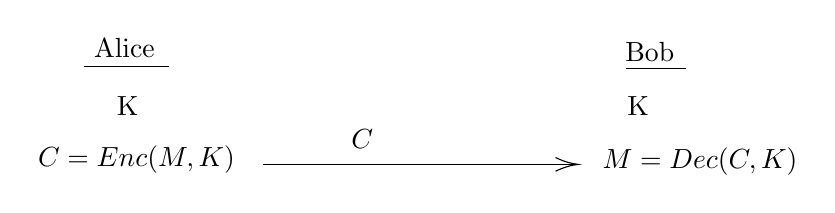
\begin{tikzpicture}[x=0.75pt,y=0.75pt,yscale=-1,xscale=1]
        \draw (157,264.6) -- (198,264.6);
        \draw (418,265.6) -- (447,265.6);
        \draw (243,311.6) -- (395,311.6);
        \draw [shift={(395,311.6)}, rotate = 180] (10.93,-3.29) .. controls (6.95,-1.4) and (3.31,-0.3) .. (0,0) .. controls (3.31,0.3) and (6.95,1.4) .. (10.93,3.29);
        
        \draw (157,246) node [anchor=north west] {Alice};
        \draw (413,248) node [anchor=north west] {Bob};
        \draw (168,274) node [anchor=north west] {K};
        \draw (414,274) node [anchor=north west] {K};
        \draw (281,290) node [anchor=north west] {$C$};
        \draw (130,298) node [anchor=north west] {$C = Enc(M, K)$};
        \draw (402,299) node [anchor=north west] {$M = Dec(C,K)$};
    \end{tikzpicture}
\end{center}    
Alice can encrypt a message and send it to Bob and Bob can decrypt the ciphertext. The problem here is that the secret key has to be same with Alice and Bob. Otherwise, the decryption will never give the correct plaintext. The problem lies in sharing the secret key. Before 1976, there was only one mechanism to share this secret key; which is, you have to meet the other party secretly. In 1976, Diffie and Hellman proposed a Key Exchange mechanism and with their results, the domain of Public Key Cryptography began. It was published in IEEE Transactions on Information Theory.\\
\newline
Let us first recall the concept of Group and a cyclic group before going further in the Diffie and Hellman Key Exchange Algorithm. A set G along with an binary operation, (G, *) is called to be Group if it satisfies the following properties:
\begin{enumerate}
    \item The operation * is closed under G, that is, if $a, b \in G$, then $a * b \in G$.
    \item $*$ is associative on G, that is, $a * (b * c) = (a * b) * c$ $ \forall$ $ a,b,c \in G$
    \item There is an element $e \in G$ called the Identity Element, such that $a * e = a = e * a$ $\forall$ $a \in G$.
    \item For each $a \in G$, there exists an element $a^{-1} \in G$, called the inverse of $a$, such that $a * a^{-1} = e = a^{-1} * a$ $\forall$ $a \in G$. 
\end{enumerate}
(G, *) is a cyclic group if every element in G can be generated using only one element $g \in G$, that is,
\begin{center}
    $\forall a \in G$ $ \exists$ $g \in G,$ such that $a = g^i,$ where $i \in Z$.
\end{center}
The element $g$ is called the generator of G, and is denoted as $G = \langle g \rangle$.\\
\newline
Now, according to Diffie and Hellman Key Exchange Algorithm, Alice and Bob will agree on one cyclic group (G, *) over a public communication. It means that via a public communication, they will agree that they both will use the cyclic group $(G, *)$ whose generator is $g$.

\begin{center}
    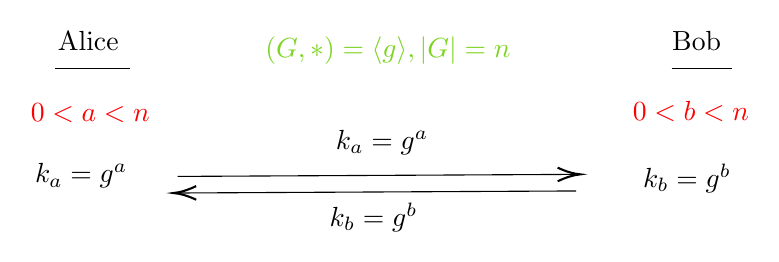
\begin{tikzpicture}[x=0.75pt,y=0.75pt,yscale=-1,xscale=1]
        \draw (150,44.4) -- (186,44.4) ;
        \draw (447,44.4) -- (476,44.4) ;
        \draw (209,96.4) -- (401,95.41) ;
        \draw [shift={(403,95.4)}, rotate = 179.7] [color={rgb, 255:red, 0; green, 0; blue, 0 } ][line width=0.75] (10.93,-3.29) .. controls (6.95,-1.4) and (3.31,-0.3) .. (0,0) .. controls (3.31,0.3) and (6.95,1.4) .. (10.93,3.29) ;
        \draw (209,104.39) -- (401,103.4) ;
        \draw [shift={(207,104.4)}, rotate = 359.7] [color={rgb, 255:red, 0; green, 0; blue, 0 } ][line width=0.75] (10.93,-3.29) .. controls (6.95,-1.4) and (3.31,-0.3) .. (0,0) .. controls (3.31,0.3) and (6.95,1.4) .. (10.93,3.29) ;
        \draw (150,25) node [anchor=north west][inner sep=0.75pt] [align=left] {Alice};
        \draw (446,25) node [anchor=north west][inner sep=0.75pt] [align=left] {Bob};
        \draw (139,89) node [anchor=north west][inner sep=0.75pt] [align=left] {$k_a = g^a$};
        \draw (432,89) node [anchor=north west][inner sep=0.75pt] [align=left] {$k_b = g^b$};
        \draw (137,60) node [anchor=north west][inner sep=0.75pt] [align=left] {\textcolor[rgb]{1,0,0}{$0 < a < n $}};
        \draw (427,59) node [anchor=north west][inner sep=0.75pt] [align=left] {\textcolor[rgb]{1,0,0}{$0 < b < n$}};
        \draw (284,73) node [anchor=north west][inner sep=0.75pt] [align=left] {$k_a = g^a$};
        \draw (281,108) node [anchor=north west][inner sep=0.75pt] [align=left] {$k_b = g^b$};
        \draw (250,28) node [anchor=north west][inner sep=0.75pt] [align=left] {\textcolor[rgb]{0.49,0.83,0.13}{$(G, *) = \langle g\rangle, |G| = n$}};
    \end{tikzpicture}
\end{center}

The part that is written with green colour in the figure above is public where as the part written in red is secret to the person on whose side it is written. Alice selects a number $a$ such that $0 < a < n $ and keeps it secret to herself. Similarly, Bob selects a number $b$ such that $0 < b < n $ and keeps it secret to himself. Alice will compute $k_a = g^a$ and send it to Bob and Bob will compute $k_a = g^a$ and send it to Alice over the public channel. That is, Alice is making $k_a$ public and Bob is making $k_b$ public. Now, Alice and Bob have the following data with them.
\begin{center}
    \tikzset{every picture/.style={line width=0.75pt}}
    \begin{tikzpicture}[x=0.75pt,y=0.75pt,yscale=-1,xscale=1]
        \draw (149,183.4) -- (185,183.4) ;
        \draw (310,184.4) -- (339,184.4) ;
        \draw (149,164) node [anchor=north west][inner sep=0.75pt] [align=left] {Alice};
        \draw (309,165) node [anchor=north west][inner sep=0.75pt] [align=left] {Bob};
        \draw (157,190) node [anchor=north west][inner sep=0.75pt] [align=left] {\textcolor[rgb]{1,0,0}{a }};
        \draw (315,191) node [anchor=north west][inner sep=0.75pt] [align=left] {\textcolor[rgb]{1,0,0}{b }};
        \draw (156,213) node [anchor=north west][inner sep=0.75pt] [align=left] {\textcolor[rgb]{0.49,0.83,0.13}{g }};
        \draw (314,215) node [anchor=north west][inner sep=0.75pt] [align=left] {\textcolor[rgb]{0.49,0.83,0.13}{g }};
        \draw (138,240) node [anchor=north west][inner sep=0.75pt] [align=left] {\textcolor[rgb]{0.49,0.83,0.13}{$k_b = g^b$}};
        \draw (297,239) node [anchor=north west][inner sep=0.75pt] [align=left] {\textcolor[rgb]{0.49,0.83,0.13}{$k_a = g^a$}};
    \end{tikzpicture}
\end{center}

Now, since, $g^a$ and $g^b$ belongs to same cyclic group. Given $g^b$, if we have $a$, then we can compute ${(g^b)}^a$. Therefore, Alice will compute ${(g^b)}^a$ and Bob will compute ${(g^a)}^b$. Therefore, Alice now has $g^{ba}$ and Bob has $g^{ab}$. Since, $a$ and $b$ are integers, therefore,
\begin{center}
    $a\cdot b = b\cdot a$\\
    $\implies g^{ba} = g^{ab}$
\end{center}
Hence, Alice and Bob have same element $g^{ab}$. They can use this element to be their secret key and start the communication using the symmetric key encryption algorithms. The same key generated by Alice and Bob, that is, $g^{ab}$ is called the Shared Secret Key.\\
\newline
We can see that Alice and Bob are exchanging some data over the public channel and they are able to establish a secret key. Since, $a$ and $b$ are only known to Alice and Bob respectively, that is, they are not shared publicly, hence, they are known as secret keys. However, $k_a = g^a$ and $k_b = g^b$ are shared by Alice and Bob to each other over a public channel. Hence, they are made public and are known as public keys. Both the parties have two keys, one public key and one secret key. Note that there may be some technique to compute $a (b)$ from $g^a (g^b)$, but since Alice (Bob) is not sharing $a (b)$, we are assuming that it is secret key for Alice(Bob).\\
\newline
Now, if we don't know the secret key of Alice (a), even if we know $g^a$ and $g^b$, we will not be able to compute $g^{ab}$, which is the key used for communication between Alice and Bob. That means, without knowing the secret key of Alice or Bob, we will not get the shared secret key used for communication between Alice or Bob.\\
\newline
Now, we have $g^x$ as public key and $x$ as secret key. If we have a very good cyclic group (G, *), based on the properties of the group, finding $x$ from $g^x$ is computationally difficult. It is possible theoretically, but the amount of time it requires is exponential. This hard problem is known as Discrete Log Problem. Since, finding $x$ from $g^x$ for a good group is computationally hard and we are using this group for establishing the shared secret key, then the key establishment mechanism will be secure. Therefore, the security of Diffie-Hellman Key Exchange Algorithm relies on the fact that Discrete Log Problem is hard for certain groups.\\
\newline
One obvious way to compute $x$ from $g^x$, as we know $G, g$ and $g^x$, is to compute $g^i$ for $1 \leq i \leq n-1$ and return $i$ if we get $g^i = g^x$.
\begin{center}
    \begin{algorithm}
    \caption{Brute Force Algorithm to find $x$ from $g^x$}
        \For{$i = 2$ to $N-1$}{
            \If{$g^i == g^x$}{
            t = i;\\
            break;
            }
        }    
    \end{algorithm}
\end{center}
The complexity here will be equal to the size of the set G, i.e $|G|$. Let us say our group contains $2^{512} - 1$ elements, then getting $x$ using this mechanism is impossible. The loop in this case will never terminate in practical time. Therefore, for the Discrete Log Problem to be hard on a group (G, *), the group must follow certain properties. These properties are mention below:
\begin{enumerate}
    \item Size of the set G, i.e $|G|$, should be very large.
    \item The group operation $*$ must be chosen carefully. Even if the group size is very large, you can still study the properties of the group operation and can find $x$ from $g^x$ very easily for certain group operators. For example, consider the cyclic group $G = (Z_p, +_p)$, p is a very large prime number and $G = \langle g \rangle$. If we try to compute $g^i$, it will be equal to:
    \begin{center}
        $g^i = g +_p g +_p ..... +_p g$\\
        $g^i = i\cdot g$
    \end{center}
    So, if we have generator of G, i.e $g$, $g^i$ can be easily computed. Now, if we know $g^i$, finding $i$ will be very easy and we will not have to search for $i$ exhaustively. Multiplying both the sides with $g^{-1}$ will give us:
    \begin{center}
        $i = g^{-1} \cdot g^i$ mod p
    \end{center}
    We know $g^i$ and we can compute $g^{-1}$ in polynomial time using the Extended Euclidean Algorithm, which will definitely hold true because gcd(i, p) = 1 as p is prime. Hence, $+_p$ is not a good group operation.
\end{enumerate}

\subsection{Man in the Middle Attack on Diffie-Hellman Key Exchange Algorithm}
Man in the Middle means there is a person who is listening to your communication and he has control over the data. Suppose you are writing a letter to your friend. You write the letter, put it in an envelope and visit the nearby post office to send it to your friend. Now, the responsibility of the post office is to transfer the letter to your friend. If the middle man, i.e. the post office, is corrupted, there will be problems and your message can be read or can be changed by the post office. In Whatsapp, you exchange certain data with its server, the server, in turn, send it to the intended person. If the Whatsapp server is corrupted, your data can be leaked.\\
\newline
Let's try to understand the Man in the Middle Attack on the Diffie-Hellman Key Exchange Algorithm.
\begin{center}
    \tikzset{every picture/.style={line width=0.75pt}}         
    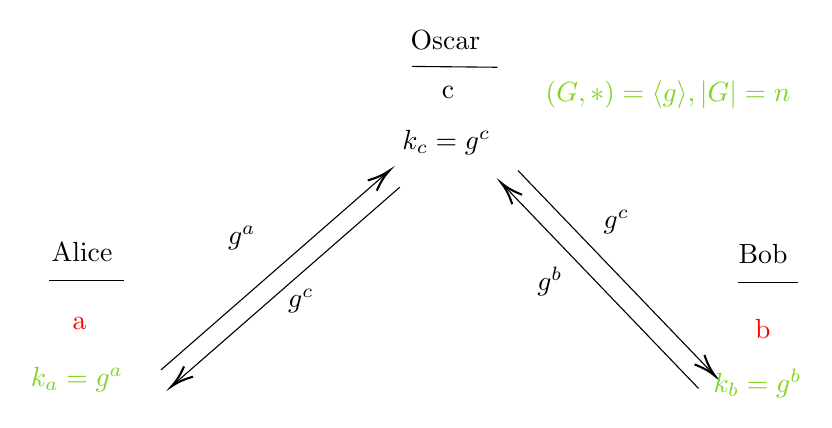
\begin{tikzpicture}[x=0.75pt,y=0.75pt,yscale=-1,xscale=1]
        \draw    (108,147.4) -- (144,147.4) ;
        \draw    (440,148.4) -- (469,148.4) ;
        \draw    (283,44.4) -- (324,44.8) ;
        \draw    (162,190.6) -- (270.49,95.92) ;
        \draw [shift={(272,94.6)}, rotate = 138.89] [color={rgb, 255:red, 0; green, 0; blue, 0 }  ][line width=0.75]    (10.93,-3.29) .. controls (6.95,-1.4) and (3.31,-0.3) .. (0,0) .. controls (3.31,0.3) and (6.95,1.4) .. (10.93,3.29)   ;
        \draw    (168.51,197.28) -- (277,102.6) ;
        \draw [shift={(167,198.6)}, rotate = 318.89] [color={rgb, 255:red, 0; green, 0; blue, 0 }  ][line width=0.75]    (10.93,-3.29) .. controls (6.95,-1.4) and (3.31,-0.3) .. (0,0) .. controls (3.31,0.3) and (6.95,1.4) .. (10.93,3.29)   ;
        \draw    (334,94.6) -- (427.62,192.16) ;
        \draw [shift={(429,193.6)}, rotate = 226.18] [color={rgb, 255:red, 0; green, 0; blue, 0 }  ][line width=0.75]    (10.93,-3.29) .. controls (6.95,-1.4) and (3.31,-0.3) .. (0,0) .. controls (3.31,0.3) and (6.95,1.4) .. (10.93,3.29)   ; 
        \draw    (327.38,102.04) -- (421,199.6) ;
        \draw [shift={(326,100.6)}, rotate = 46.18] [color={rgb, 255:red, 0; green, 0; blue, 0 }  ][line width=0.75]    (10.93,-3.29) .. controls (6.95,-1.4) and (3.31,-0.3) .. (0,0) .. controls (3.31,0.3) and (6.95,1.4) .. (10.93,3.29)   ;
        
        \draw (108,128) node [anchor=north west][inner sep=0.75pt]   [align=left] {Alice};
        \draw (439,129) node [anchor=north west][inner sep=0.75pt]   [align=left] {Bob};
        \draw (346,50) node [anchor=north west][inner sep=0.75pt]   [align=left] {\textcolor[rgb]{0.49,0.83,0.13}{$(G, *) = \langle g\rangle, |G| = n$}};
        \draw (281,26) node [anchor=north west][inner sep=0.75pt]   [align=left] {Oscar};
        \draw (118,164) node [anchor=north west][inner sep=0.75pt]   [align=left] {\textcolor[rgb]{1,0,0}{a}};
        \draw (98,188) node [anchor=north west][inner sep=0.75pt]   [align=left] {\textcolor[rgb]{0.49,0.83,0.13}{$k_a = g^a$}};
        \draw (447,165) node [anchor=north west][inner sep=0.75pt]   [align=left] {\textcolor[rgb]{1,0,0}{b}};
        \draw (427,189) node [anchor=north west][inner sep=0.75pt]   [align=left] {\textcolor[rgb]{0.49,0.83,0.13}{$k_b = g^b$}};
        \draw (277,74) node [anchor=north west][inner sep=0.75pt]   [align=left] {$k_c = g^c$};
        \draw (296,53) node [anchor=north west][inner sep=0.75pt]   [align=left] {c};
        \draw (193,120) node [anchor=north west][inner sep=0.75pt]   [align=left] {$g^a$};
        \draw (222,150.6) node [anchor=north west][inner sep=0.75pt]   [align=left] {$g^c$};
        \draw (374,112.6) node [anchor=north west][inner sep=0.75pt]   [align=left] {$g^c$};
        \draw (342,139.6) node [anchor=north west][inner sep=0.75pt]   [align=left] {$g^b$};
    \end{tikzpicture}
\end{center} 

Here, Oscar can capture the communication between Alice and Bob. Suppose if Alice has sent some message to Bob. Oscar can capture this message and can send a different message to Bob. Suppose Alice has sent $g^a$ to Bob. Oscar will compute $g^c$ as g and G are public. Oscar will intercept the $g^a$ sent by Alice to Bob and send $g^c$ to Bob. Since, Bob doesn't have any mechanism for authenticating that the message is coming from Alice, Bob will believe that Alice has sent her public key to him. However, this is not the case, Bob has actually recieved $g^c$ (not $g^a$).\\
Bob will share his public key $g^b$ to Alice. Again, Oscar will intercept this message and send $g^c$ to Alice. Alice, again, doesn't have any mechanism to check if it is coming from Bob or not, so she will accept it.\\
With the data that Alice has, she can compute:
\begin{center}
    ${(g^c)}^a = g^{ac}$
\end{center}
With the data that Bob has, he can compute:
\begin{center}
    ${(g^c)}^b = g^{bc}$
\end{center}
and with the data that Oscar have, he can compute:
\begin{center}
    ${(g^a)}^c = g^{ac}$ \\ 
    ${(g^b)}^c = g^{bc}$
\end{center}
Now, Oscar has two shared secret keys, one is same with Alice and the other is same with Bob. Alice and Bob will begin the communication as they are unaware about the middle man. Suppose Alice has sent a message to Bob.
\begin{center}
    \tikzset{every picture/.style={line width=0.75pt}}     
    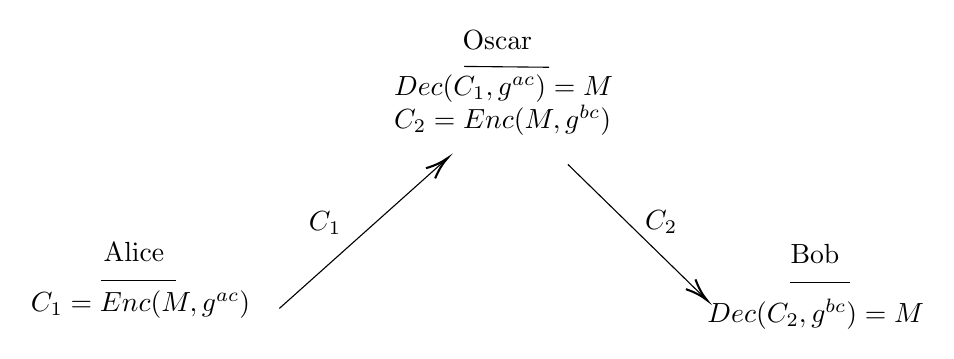
\begin{tikzpicture}[x=0.75pt,y=0.75pt,yscale=-1,xscale=1]
        \draw    (107,400.4) -- (143,400.4) ;
        \draw    (439,401.4) -- (468,401.4) ;
        \draw    (282,297.4) -- (323,297.8) ;
        \draw    (193,414) -- (272.51,342.93) ;
        \draw [shift={(274,341.6)}, rotate = 138.21] [color={rgb, 255:red, 0; green, 0; blue, 0 }  ][line width=0.75]    (10.93,-3.29) .. controls (6.95,-1.4) and (3.31,-0.3) .. (0,0) .. controls (3.31,0.3) and (6.95,1.4) .. (10.93,3.29)   ;
        \draw    (332,344.6) -- (397.57,408.6) ;
        \draw [shift={(399,410)}, rotate = 224.31] [color={rgb, 255:red, 0; green, 0; blue, 0 }  ][line width=0.75]    (10.93,-3.29) .. controls (6.95,-1.4) and (3.31,-0.3) .. (0,0) .. controls (3.31,0.3) and (6.95,1.4) .. (10.93,3.29)   ;
        
        \draw (107,381) node [anchor=north west][inner sep=0.75pt]   [align=left] {Alice};
        \draw (438,382) node [anchor=north west][inner sep=0.75pt]   [align=left] {Bob};
        \draw (280,279) node [anchor=north west][inner sep=0.75pt]   [align=left] {Oscar};
        \draw (206,366) node [anchor=north west][inner sep=0.75pt]   [align=left] {$C_1$};
        \draw (368,365.6) node [anchor=north west][inner sep=0.75pt]   [align=left] {$C_2$};
        \draw (247,300) node [anchor=north west][inner sep=0.75pt]   [align=left] {$Dec(C_1, g^{ac}) = M$\\$C_2 = Enc(M, g^{bc})$};
        \draw (72,404) node [anchor=north west][inner sep=0.75pt]   [align=left] {$C_1 = Enc(M, g^{ac})$};
        \draw (398,408) node [anchor=north west][inner sep=0.75pt]   [align=left] {$Dec(C_2, g^{bc}) = M$};
    \end{tikzpicture}
\end{center}

Alice will encrypt the message using $g^{ac}$ and send it. Oscar will receive this message and decrypt it using $g^{ac}$. Oscar will get the original message sent by Alice. Now, Oscar will encrypt this message using $g^{bc}$ and send it to Bob. Bob on receiving the message will decrypt it using $g^{bc}$ and will receive the original message sent by Alice. Both Alice and Bob will be unaware of the fact that Oscar is receiving all the communication between them. This is known as Man in the Middle Attack on Diffie-Hellman Key Exchange Algorithm.\\
\newline
In Whatsapp or Telegram, Diffie-Hellman Key Exchange is used. This exchange is performed by the middle person, i.e the Whatsapp or Telegram. If they want they can do anything with the data. However, there are certain mechanisms which they implement to provide security.\\
\newline
If we wish to compute the shared secret key $g^{ab}$, we have to compute $g^a$ and $g^b$ where $|G|$ is large and also $a$ and $b$ should be large. In fact, if you will use any pseudo-random selector from 1 to (n-1), it is highly guaranteed that it will be in the middle of 1 and (n-1). Hence, if $|G| = 2^{512}$, then $a$ and $b$ will be in the order of 256 bits. The problem here is how to compute $g^a$ and $g^b$ efficiently. It is not possible to compute $g^a$ and $g^b$ by running a loop and multiplying by $g$ in each iteration. This is practically impossible. Therefore, to compute $g^a$ and $g^b$, we use the Square and Multiply Algorithm. According to the algorithm, suppose we want to calculate $x^c$. The binary representation of $c$ is $c_{l-1}\hdots c_1, c_0$. Then, \\
 \vspace{3mm}
$c = \Sigma_{i = 0}^{l-1} c_i \cdot 2^i$\\
\vspace{3mm}
$x^c = x^{\Sigma_{i = 0}^{l-1} c_i \cdot 2^i} = \Pi_{i = 0}^{l-1} x^{c_i \cdot 2^i}$\\
\vspace{3mm}
$x^c = x^{c_0\cdot 2^0}\hdots x^{c_{l-1}\cdot 2^{l-1}}$\\
These are just $log(c)$ multiplications, hence, we can compute $x^c$ in logarithmic time of c.
\begin{center}
    \begin{algorithm}
    \caption{Square and Multiply Algorithm to find $x^c$}
        \textbf{Input:} x and c\\
        Z = 1;\\
        \For{$i = l - 1$ to $N0$}{
            $Z = Z^2$;\\
            \If{$c_i == 1$}{
                Z = Z * x;\\
            }
        }
        return Z;
    \end{algorithm}
\end{center}
Let us take and example and calculate $3^5$. Therefore, x = 3 and c = 5 = $(101)_2$. Initially Z = 1, i = 2 (since l = 3). First iteration of for loop, $Z = Z^2 = 1$, since $c_2 = 1$, $Z = Z * x = 3$. Second iteration of for loop, Z = 3, i = 1. $Z = Z^2 = 9$, since $c_1 = 0$, Z will not be multiplied by x. Last iteration of for loop, Z = 9, i = 0. $Z = Z^2 = 81$, since $c_0 = 1$, $Z = Z * x = 81 * 3 = 243$. Z = 243 = $3^5$ is returned.\\
\newline
Using the Square and Multiply Algorithm $g^a$ and $g^b$ can be computed efficiently in $log(a)$ and $log(b)$ time complexity respectively.\\
\newline

\begin{center}
    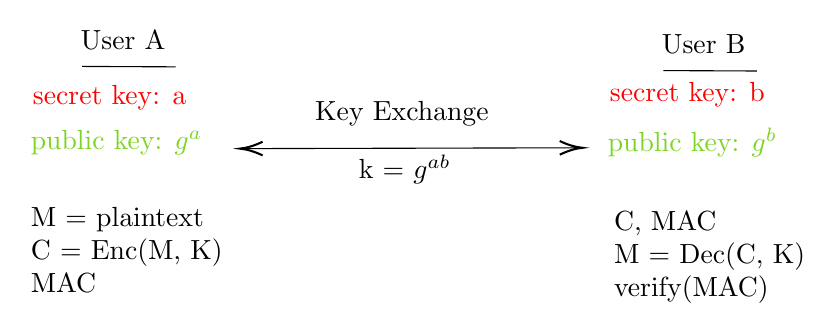
\begin{tikzpicture}[x=0.75pt,y=0.75pt,yscale=-1,xscale=1]
        \draw (161,476.4) -- (206,476.6) ;
        \draw (441,478.4) -- (486,478.6) ;
        \draw (239,516) -- (400,515.6) ;
        \draw [shift={(402,515.6)}, rotate = 179.86] [color={rgb, 255:red, 0; green, 0; blue, 0 } ][line width=0.75] (10.93,-3.29) .. controls (6.95,-1.4) and (3.31,-0.3) .. (0,0) .. controls (3.31,0.3) and (6.95,1.4) .. (10.93,3.29) ;
        \draw [shift={(237,516)}, rotate = 359.86] [color={rgb, 255:red, 0; green, 0; blue, 0 } ][line width=0.75] (10.93,-3.29) .. controls (6.95,-1.4) and (3.31,-0.3) .. (0,0) .. controls (3.31,0.3) and (6.95,1.4) .. (10.93,3.29) ;
        
        \draw (159,458) node [anchor=north west][inner sep=0.75pt] [align=left] {User A};
        \draw (136,484) node [anchor=north west][inner sep=0.75pt] [align=left] {\textcolor[rgb]{1,0,0}{secret key: a}};
        \draw (135,506) node [anchor=north west][inner sep=0.75pt] [align=left] {\textcolor[rgb]{0.49,0.83,0.13}{public key: $g^a$}};
        \draw (439,460) node [anchor=north west][inner sep=0.75pt] [align=left] {User B};
        \draw (414,483) node [anchor=north west][inner sep=0.75pt] [align=left] {\textcolor[rgb]{1,0,0}{secret key: b}};
        \draw (413,505) node [anchor=north west][inner sep=0.75pt] [align=left] {\textcolor[rgb]{0.49,0.83,0.13}{public key: $g^b$}};
        \draw (272,492) node [anchor=north west][inner sep=0.75pt] [align=left] {Key Exchange};
        \draw (293,518) node [anchor=north west][inner sep=0.75pt] [align=left] {k = $g^{ab}$};
        \draw (135,543) node [anchor=north west][inner sep=0.75pt] [align=left] {M = plaintext\\C = Enc(M, K)\\MAC};
        \draw (416,545) node [anchor=north west][inner sep=0.75pt] [align=left] {C, MAC\\M = Dec(C, K)\\verify(MAC)}; 
    \end{tikzpicture}
\end{center}

Now, if we have a Man in the Middle Attack, then we can have a communication setup where the MAC can also be incorporated. The MAC authenticates the source of the message as well as the correctness of the message. So, now we can authenticate the source, hence, the Man in the Middle Attack will not be possible now.

\subsection{RSA (Rivest Shamir Adleman) Encryption}
It is the first public key encryption algorithm. Before beginning any discussion on RSA encryption, let's first recall a few concepts.
\begin{itemize}
    \item The Euler's Totient Function $\phi(n)$ denotes the number of integers less than n that are co-prime to n, i.e number of x such that gcd(x, n) = 1 where $1 \leq x \leq n-1$
    \item Let there be a set $S = \{x$ mod m$\}$ such that $|S| = m$.
    \begin{center}
        $S = \{r_1, r_2,\hdots, r_m\}$
    \end{center}
    All the elements in the set S are unique (usually they are from 0 to m-1). Assume an integer $a$ such that $gcd(a, m) = 1$. Let's say that there is another set $S_1$ such that,
    \begin{center}
        $S_1 = \{ar_1$ mod $m, ar_2$ mod m$,\hdots, ar_m$ mod $m\}$
    \end{center}
    Since, $\{r_1, r_2,\hdots, r_m\}$ are different elements and gcd(a, m) = 1, it can be concluded that $\{ar_1$ mod $m, ar_2$ mod m$,\hdots, ar_m$ mod $m\}$ will also be $m$ unique elements. This can be proves using contradiction. Suppose, if $ar_i = ar_j$ for $r_i \neq r_j$. Therefore,
    \begin{center}
        $ar_i \equiv ar_j$ mod $m$
    \end{center}
    Since, gcd(a, m) = 1, therfore, $1 = ab + ms$( from Bezout's Identity). Therefore, there exists an integer $b$ such that $ab \equiv 1$ mod m. The value of b is known as multiplicative inverse of $a$ and it can be found using Extended Euclidean Algorithm.
    Therefore, on multiplying the above equation by b on both sides gives us,
    \begin{center}
        $b\cdot a\cdot r_i \equiv b\cdot a \cdot r_j$ mod $m$\\
        \vspace{3mm}
        $r_i \equiv r_j$ mod m    ($\because ab \equiv 1$ mod m)
    \end{center}
    Hence, it is a contradiction to our initial assumption that $r_i \neq r_j$. Hence, elements in the set $S_1$ will be unique iff gcd(a, m) = 1.
\end{itemize}



\end{document}
